%% abtex2-modelo-trabalho-academico.tex, v-1.9.6 laurocesar
%% Copyright 2012-2016 by abnTeX2 group at http://www.abntex.net.br/ 
%%
%% This work may be distributed and/or modified under the
%% conditions of the LaTeX Project Public License, either version 1.3
%% of this license or (at your option) any later version.
%% The latest version of this license is in
%%   http://www.latex-project.org/lppl.txt
%% and version 1.3 or later is part of all distributions of LaTeX
%% version 2005/12/01 or later.
%%
%% This work has the LPPL maintenance status `maintained'.
%% 
%% The Current Maintainer of this work is the abnTeX2 team, led
%% by Lauro César Araujo. Further information are available on 
%% http://www.abntex.net.br/
%%
%% This work consists of the files abntex2-modelo-trabalho-academico.tex,
%% abntex2-modelo-include-comandos and abntex2-modelo-references.bib
%%

% ------------------------------------------------------------------------
% ------------------------------------------------------------------------
% abnTeX2: Modelo de Trabalho Academico (tese de doutorado, dissertacao de
% mestrado e trabalhos monograficos em geral) em conformidade com 
% ABNT NBR 14724:2011: Informacao e documentacao - Trabalhos academicos -
% Apresentacao
% ------------------------------------------------------------------------
% ------------------------------------------------------------------------

\documentclass[
	% -- opções da classe memoir --
	12pt,				% tamanho da fonte
	openright,			% capítulos começam em pág ímpar (insere página vazia caso preciso)
	twoside,			% para impressão em recto e verso. Oposto a oneside
	a4paper,			% tamanho do papel. 
	% -- opções da classe abntex2 --
	%chapter=TITLE,		% títulos de capítulos convertidos em letras maiúsculas
	%section=TITLE,		% títulos de seções convertidos em letras maiúsculas
	%subsection=TITLE,	% títulos de subseções convertidos em letras maiúsculas
	%subsubsection=TITLE,% títulos de subsubseções convertidos em letras maiúsculas
	% -- opções do pacote babel --
	english,			% idioma adicional para hifenização
	french,				% idioma adicional para hifenização
	spanish,			% idioma adicional para hifenização
	brazil				% o último idioma é o principal do documento
	]{abntex2}

% ---
% Pacotes básicos 
% ---
\usepackage{times}				% Usa a fonte Times New Roman		
\usepackage[T1]{fontenc}		% Selecao de codigos de fonte.
\usepackage[utf8]{inputenc}		% Codificacao do documento (conversão automática dos acentos)
\usepackage{lastpage}			% Usado pela Ficha catalográfica
\usepackage{indentfirst}		% Indenta o primeiro parágrafo de cada seção.
\usepackage{color}				% Controle das cores
\usepackage{graphicx}			% Inclusão de gráficos
\usepackage{microtype} 			% para melhorias de justificação
\usepackage{longtable}
\usepackage{booktabs}
\usepackage{graphicx}
\usepackage{multirow}
\usepackage{float}
\usepackage{tabularx}
\usepackage{pdflscape}
% ---
		
% ---
% Pacotes adicionais, usados apenas no âmbito do Modelo Canônico do abnteX2
% ---
\usepackage{lipsum}				% para geração de dummy text
% ---

% ---
% Pacotes de citações
% ---
\usepackage[brazilian,hyperpageref]{backref}	 % Paginas com as citações na bibl
\usepackage[alf]{abntex2cite}	% Citações padrão ABNT

% --- 
% CONFIGURAÇÕES DE PACOTES
% --- 

% ---
% Configurações do pacote backref
% Usado sem a opção hyperpageref de backref
\renewcommand{\backrefpagesname}{Citado na(s) página(s):~}
% Texto padrão antes do número das páginas
\renewcommand{\backref}{}
% Define os textos da citação
\renewcommand*{\backrefalt}[4]{
	\ifcase #1 %
		Nenhuma citação no texto.%
	\or
		Citado na página #2.%
	\else
		Citado #1 vezes nas páginas #2.%
	\fi}%
% ---

% ---
% Informações de dados para CAPA e FOLHA DE ROSTO
% ---
\titulo{Pobreza multidimensional e os beneficiários do BPC: uma comparação entre estratos de renda per capita}
\autor{Tamara Vaz de Moraes Santos}
\local{Brasília - DF}
\data{2017}
\orientador{Ana Carolina Pereira Zoghbi}
\instituicao{%
  Universidade de Brasília -- UnB
  \par
  Faculdade de Economia Administração e Contabilidade -- FACE
  \par
  Departamento de Economia}
\tipotrabalho{Monografia)}
% O preambulo deve conter o tipo do trabalho, o objetivo, 
% o nome da instituição e a área de concentração 
\preambulo{Monografia apresentada ao Departamento de Economia da Universidade de Brasília para obtenção do grau de Bacharel em Economia}
% ---


% ---
% Configurações de aparência do PDF final

% alterando o aspecto da cor azul
\definecolor{blue}{RGB}{41,5,195}

% informações do PDF
\makeatletter
\hypersetup{
     	%pagebackref=true,
		pdftitle={\@title}, 
		pdfauthor={\@author},
    	pdfsubject={\imprimirpreambulo},
	    pdfcreator={LaTeX with abnTeX2},
		pdfkeywords={abnt}{latex}{abntex}{abntex2}{trabalho acadêmico}, 
		colorlinks=true,       		% false: boxed links; true: colored links
    	linkcolor=blue,          	% color of internal links
    	citecolor=blue,        		% color of links to bibliography
    	filecolor=magenta,      		% color of file links
		urlcolor=blue,
		bookmarksdepth=4
}
\makeatother
% --- 

% --- 
% Espaçamentos entre linhas e parágrafos 
% --- 

% O tamanho do parágrafo é dado por:
\setlength{\parindent}{1.3cm}

% Controle do espaçamento entre um parágrafo e outro:
\setlength{\parskip}{0.2cm}  % tente também \onelineskip

% ---
% compila o indice
% ---
\makeindex
% ---

% ----
% Início do documento
% ----
\begin{document}

% Seleciona o idioma do documento (conforme pacotes do babel)
%\selectlanguage{english}
\selectlanguage{brazil}

% Retira espaço extra obsoleto entre as frases.
\frenchspacing 

% ----------------------------------------------------------
% ELEMENTOS PRÉ-TEXTUAIS
% ----------------------------------------------------------
% \pretextual

% ---
% Capa
% ---
\imprimircapa
% ---

% ---
% Folha de rosto
% (o * indica que haverá a ficha bibliográfica)
% ---
\imprimirfolhaderosto*
% ---

% ---
% Inserir a ficha bibliografica
% ---

% Isto é um exemplo de Ficha Catalográfica, ou ``Dados internacionais de
% catalogação-na-publicação''. Você pode utilizar este modelo como referência. 
% Porém, provavelmente a biblioteca da sua universidade lhe fornecerá um PDF
% com a ficha catalográfica definitiva após a defesa do trabalho. Quando estiver
% com o documento, salve-o como PDF no diretório do seu projeto e substitua todo
% o conteúdo de implementação deste arquivo pelo comando abaixo:
%
% \begin{fichacatalografica}
%     \includepdf{fig_ficha_catalografica.pdf}
% \end{fichacatalografica}

% ---



% ---
% Inserir folha de aprovação
% ---

% Isto é um exemplo de Folha de aprovação, elemento obrigatório da NBR
% 14724/2011 (seção 4.2.1.3). Você pode utilizar este modelo até a aprovação
% do trabalho. Após isso, substitua todo o conteúdo deste arquivo por uma
% imagem da página assinada pela banca com o comando abaixo:
%
% \includepdf{folhadeaprovacao_final.pdf}
%
\begin{folhadeaprovacao}

  \begin{center}
    {\ABNTEXchapterfont\large\imprimirautor}

    \vspace*{\fill}\vspace*{\fill}
    \begin{center}
      \ABNTEXchapterfont\bfseries\Large\imprimirtitulo
    \end{center}
    \vspace*{\fill}
    
    \hspace{.45\textwidth}
    \begin{minipage}{.5\textwidth}
        \imprimirpreambulo
    \end{minipage}%
    \vspace*{\fill}
   \end{center}
        
   Trabalho aprovado. \imprimirlocal, 11 de julho de 2017:

   \assinatura{\textbf{Profª. Drª. \imprimirorientador} \\ Orientador} 
   \assinatura{\textbf{Profª. Drª. Déborah Oliveira Martins dos Reis} \\ Banca Examinadora}
   %\assinatura{\textbf{Professor} \\ Convidado 3}
   %\assinatura{\textbf{Professor} \\ Convidado 4}
      
   \begin{center}
    \vspace*{0.5cm}
    {\large\imprimirlocal}
    \par
    {\large\imprimirdata}
    \vspace*{1cm}
  \end{center}
  
\end{folhadeaprovacao}
% ---



% ---
% Agradecimentos
% ---
\begin{agradecimentos}


\end{agradecimentos}
% ---
% ---
% RESUMOS
% ---

% resumo em português
\setlength{\absparsep}{18pt} % ajusta o espaçamento dos parágrafos do resumo
\begin{resumo}
 Este trabalho compara a pobreza multidimensional familiar dos potenciais beneficiários do Benefício de Prestação Continuada (BPC) e da população adicional que poderia ser elegível caso o critério de renda para a elegibilidade do programa fosse modificado para até 1/2 do salário mínimo \textit{per capita}. O BPC é um benefício da Assistência Social que garante um salário mínimo mensal as pessoas com deficiência e aos idosos que tenham renda \textit{per capita} de até 1/4 do salário mínimo. O critério de 1/2 de renda \textit{per capita} tem sido adotado para as concessões do BPC por vias judiciais, sob o argumento de que o requerente que teve seu pedido negado por extrapolar o limite de renda do programa, tem condições socioeconômicas tão agravadas quando os naturalmente eleitos pelas regras atuais do benefício. As reclamações com esse teor argumentativo chegaram até o Supremo Tribunal Federal (STF) diversas vezes, embora só em 2013 o SFT tenha formado o entendimento de que outros elementos comprobatórios de miserabilidade podem ser usados para conceder judicialmente o benefício, sem no entanto estipular quais seriam esses critérios. Com isso, a lei que regulamenta o programa ficou omissa quanto aos novos critérios, e o antigo critério ainda continua válido. A principal conclusão deste trabalho é que os estratos de renda \textit{per capita} -- de até 1/4 e maior que 1/4 e até 1/2, não são diferentes em pobreza quando levadas em conta várias dimensões. Além da similaridade do índice sintético geral, os grupos também são similares nas dimensões desagregadas do índice e na distribuição das famílias por índice de pobreza. Outra conclusão relevante é que, mesmo havendo um tratamento não isonômico entre pessoas com deficiência e idosos na LOAS, esses não diferem quanto ao grau de pobreza medido pelo índice, tanto comparados dentro dos estratos quando entre os estratos.


 \textbf{Palavras-chave}: pobreza; indicador multidimensional; Benefício de prestação continuada; judicialização  da  política  pública.
\end{resumo}


% ---
% inserir lista de ilustrações
% ---
\pdfbookmark[0]{\listfigurename}{lof}
\listoffigures*
\cleardoublepage
% ---

% ---
% inserir lista de tabelas
% ---
\pdfbookmark[0]{\listtablename}{lot}
\listoftables*
\cleardoublepage
% ---

% ---
% inserir o sumario
% ---
\pdfbookmark[0]{\contentsname}{toc}
\tableofcontents*
\cleardoublepage
% ---



% ----------------------------------------------------------
% ELEMENTOS TEXTUAIS
% ----------------------------------------------------------
\textual

% ---
% Introdução
% ---
\chapter{Introdução}

O Benefício de Prestação Continuada (BPC) faz parte dos benefícios da Assistência Social previstos na Constituição Federal Brasileira de 1998. O benefício é direcionado às pessoas idosas ou com deficiência que comprovarem não possuir meios de prover a própria manutenção ou de tê-la provida por sua família. O BPC é caracterizado como não condicional, pois não depende de qualquer contribuição prévia ou contrapartida financeira por parte do beneficiário. Apesar desse benefício estar previsto no texto constitucional desde 1988, a regulamentação do programa só se deu em 1993 com a publicação da Lei Orgânica de Assistência Social (LOAS). A LOAS  A lei que regulamenta o programa entendeu como insuficiência de meios para a manutenção o limite de renda \textit{per capita} de até 1/4 de salário mínimo. 

Ao longo dos anos, diversas foram as contestações dos critérios do BPC definidos pela Lei Orgânica de Assistência social (LOAS). Um dos mais questionados, e que permaneceu inalterado desde sua concepção, foi o de insuficiência de renda. A criação de novos programas no âmbito da Assistência Social, que previam o corte de elegibilidade de até 1/2 do salário mínimo \textit{per capita}, gerou embasamento argumentativo para que o BPC fosse concedido na justiça ordinária quando a renda \textit{per capita} do requerente era de até 1/2 do salário mínimo. Em 2013 o Supremo Tribunal Federal (STF) julgou que, para o deferimento do Benefício de Prestação Continuada, podem ser consideradas outros elementos probatórios de miserabilidade além da regra de 1/4 de salário mínimo, sem decretar a nulidade critério de renda do BPC. Os demais critérios que comprovem a situação de miserabilidade do grupo familiar e da situação de vulnerabilidade carecem de regulamento e estão omitidos na Lei Orgânica de Assistência Social. Dessa forma, o critério de pobreza para a concessão do benefício se tornou subjetivo, ficando ao arbítrio das análises individual dos casos deferidos pelo judiciário. 

Esse subjetivismo introduzido ao programa pela decisão do STF se a grava ao perceber que as concessões judiciais têm crescido ao longo dos anos, e já respondem por uma parte significativa de todas concessões do benefício. Além disso, a literatura pertinente argumenta que as concessões têm um efeito perverso sobre a isonomia, já que o acesso ao judiciário é desigual, privilegiando indivíduo mais instruídos e que estão em locais onde há menor ocorrências de pobreza.

Conquanto, o entendimento do judiciário de que indivíduos com rendas mais altas podem estar na mesma, ou pior, situação de pobreza não é espúrio. A definição de pobreza como fenômeno multidimensional tem certo consenso na literatura. A existência de bens não monetário e o acesso desigual aos recursos corroboram o uso de uma análise multidimensional em detrimento da puramente monetária. Entretanto, os problemas na operacionalização dessas análises são tão expressivos quanto as críticas ao uso da insuficiência de renda para aferir a pobreza. 

O presente trabalho apresenta um esforço no sentido de avaliar se os extratos de renda \textit{per capita}, o critério de 1/4 estipulado na LOAS e o de 1/2 adotado implicitamente pelo judiciário, são de fato similares em termos de pobreza. Os dados de indivíduos e domicílio são provenientes da Pesquisa Nacional de Saúde (PNS) de 2013. A escolha da PNS como fonte de dados adveio da maior disponibilidade de indicadores dos tipos de deficiência e limitações advindas dela. O método consistiu em x etapas:

\begin{enumerate}
	\item Identificação dos preeleitos ao BPC, aplicando todas as regras de elegibilidade prevista na LOAS, exceto renda.
	\item Recriação do grupo familiar do beneficiário, mantendo apenas os indivíduos que podem entrar no cômputo da renda.
	\item Identificação e retirada das rendas provenientes do Programa Bolsa Família
	\item Cálculo da renda familiar \textit{per capita}
	\item Cálculo do índice de pobreza familiar multidimensional para cada estrado
\end{enumerate}

Esse estudo está organizado em seis seções, sendo a primeira esta introdução. Na segunda seção são apresentadas um breve histórico das concessões judiciais do BPC e suas regras de elegibilidade. O terceiro expõe a revisão de literatura sobre pobreza multidimensional. A quarta seção explicita os métodos e procedimentos necessários para a obtenção dos estratos de renda dos elegíveis ao BPC e a construção do índice de pobreza familiar multidimensional. Em seguida, na quinta seção são descritos os resultados e, por fim, a sexta apresenta as conclusões.
 
% ---


% ---
% Programa de Prestação Continuada e sua judicialização
% ---
\chapter{Programa de Prestação Continuada e concessões por vias judiciais}

	\section{BPC e regras de elegibilidade }
A Constituição de 1998 prevê, como parte da assistência social, ``a garantia de um salário mínimo de benefício mensal à pessoa portadora de deficiência e ao idoso que comprovem não possuir meios de prover à própria manutenção ou de tê-la provida por sua família, conforme dispuser a lei'' \cite[Art. 203, inciso V]{brasil1988}. Além disso, essa transferência não depende de contribuição prévia à seguridade social ou de qualquer contrapartida por parte do beneficiário. Conquanto, a política pública para essa finalidade so viria a ser regulamentada em 1993 pela Lei Orgânica Social (LOAS), definindo critérios objetivos para o recebimento do Benefício de Prestação Continuada (BPC). O benefício é coordenado pelo Ministério do Desenvolvimento Social e Combate à Fome -- MDS, operacionalizado pelo Instituto Nacional do Seguro Social -- INSS.


As regras de elegibilidade elencadas na LOAS foram redefinidas diversas vezes, a apresentada aqui será a mais atual, sendo a ultima modificação realizada pelo Decreto nº 8.805, de 7 de julho de 2016. O candidato ao benefício deve estar inscrito no Cadastro Único para Programas Sociais do Governo Federal (Cadastro Único) e se enquadrar nos seguintes critérios: ter insuficiência de meios de provimento, ser idoso ou pessoa com deficiência.
		
		 A incapacidade de provimento mínimo é definida como a pessoa que tenha renda \textit{per capita} inferior a 1/4 do salário mínimo vigente. Ademais, nos casos de concessão do benefício para pessoas com deficiências, essas não poderão exercer atividade remunerada, excedo na condição de aprendiz por um prazo máximo de dois anos. Segundo \citeonline{adriana2016}, o estabelecimento de um corte de renda para definir o limite de pobreza ser elegível é largamente utilizado nos programas governamentais, de modo a facilitar a operacionalização dos programas e evitar o tratamento não isonômico. Embora não se tenha explicitamente justificado o corte de 1/4 de renda \textit{per capita}, \citeonline{adriana2016} afirma ainda que o corte do programa advém de uma inferência da definição de salário mínimo da Constituição, que o define da seguinte forma:
		 
		 \begin{citacao}
		 	IV - salário mínimo , fixado em lei, nacionalmente unificado, capaz de atender a suas necessidades vitais básicas e às de sua família com moradia, alimentação, educação, saúde, lazer, vestuário, higiene, transporte e previdência social, com reajustes periódicos que lhe preservem o poder aquisitivo, sendo vedada sua vinculação para qualquer fim \cite[Art. 7{\textordmasculine}]{brasil1988}.
		 	
		 \end{citacao}
	 
	  Assim, o salário mínimo presumia que o valor era capaz de atender às necessidades básicas de uma família mononuclear, ou seja: pessoa, conjugue e dois filhos, corroborando o corte de 1/4 do salário mínimo instituído.
		

		Para definir a renda por pessoa do candidato ao BPC, a LOAS determina quem deve entrar no cômputo dessa renda. Para isso, é definido o conceito de grupo familiar do beneficiário. A LOAS explicita a inclusão nesse cálculo as rendas do requerente ao benefício, seu cônjuge, filhos e enteados solteiros, irmãos solteiros, os pais e, na ausência de um deles, a madrasta ou o padrasto e menores tutelados, desde que esses integrantes familiares vivam sobre o mesmo teto. Como explicitado, o conceito familiar no BPC não é definido estritamente segundo a existência de uma unidade de consumo. \citeonline{medeiros2009mudancca} afirma que a definição atual de família do programa traz distorssoes, podendo superestimar a renda de algumas famílias pobres ou subestimar a capacidade de prover o sustento de famílias que tenham filhos e irmãos casados ou demais parentes mais ricos. Como essa definição impacta diretamente o cálculo da renda \textit{per capita}, estudos já verificaram o efeito de uma mudança nesse conceito. A mudança que considere a unidade domiciliar de consumo como família, traria a exclusão e introdução de beneficiários, tendo em média efeito nulo líquido. No entanto, traria uma maior focalização do programa \cite{medeiros2009mudancca,fambpcfreitas}.
		
		O conceito de idoso é o requisito em que há menor discussão, dada a objetividade do corte de idade. A idade mínima segue atualmente o descrito no Estatuto do Idoso de 2003, considerando idoso pessoas com 65 anos ou mais \cite{lei_idoso2003}. 
		
		A  Convenção das Nações Unidas sobre os Direitos das Pessoas com Deficiência de 2006, e que foi ratificada pelo Brasil em 2008, norteou a definição de pessoa com deficiência no Benefício de Prestação Continuada. Para a Convenção, além das barreiras físicas de longo prazo que constituem a definição de pessoa com deficiência, o a deficiência deve também ser entendida em seu contexto social. Isso implica dizer que o conceito não é rígido e imutável. Assim, esse conceito deve se adequar e levar em consideração às barreiras impostas pelo estilo de vida e pelo ambiente que impeçam o indivíduo de ter igualdade de oportunidades e de participação na sociedade \cite{onu2006convention}. Em consonância com a Convenção, a LOAS avalia a pessoa com deficiência em duas etapas: a primeira verifica a deficiência do ponto de vista físico, avaliado por um exame médico; a segunda etapa avalia o grau de impedimento do indivíduo em relação ao meio, a partir de uma investigação social realizada por assistentes sociais do Instituto Nacional de Seguro Social (INSS). No entanto, não há definição dos parâmetros usados para a segunda etapa na lei. 
				
\section{Judicializações e entendimento atual}

Dentre as regras de elegibilidade definidas na LOAS, a que mais têm  gerado concessões por judicialização foi a definição de insuficiência de meios a partir do corte de renda per capita em 1/4 \cite{adriana2016}. O debate sobre o uso desse corte como único meio de aferir a pobreza do indivíduo foi diversas vezes questionada, chegando ao STF. 

Dois anos após a regulamentação do BPC, foi interposto a Ação direta de Inconstitucionalidade nº 1.232, ajuizada pelo Procurador Geral da República, que pedia a suspensão da regra de renda mínima para a concessão do BPC, com o seguinte argumento:

	\begin{citacao}
	Adota o requerente os fundamentos expostos em solicitação que lhe foi dirigida pelo órgão, no Estado de São Paulo, segundo os quais o dispositivos sob enfoque limita e restringe o direito garantido por norma constitucional (art. 2013, inc. V), com a qual, por isso, considera incompatível \cite[pag. 96 ]{acao1232}.
\end{citacao}

A ação foi julgada improcedente, prevalecendo o entendimento de que a definição de insuficiência de meios caberia somente a lei, e por isso essa seria soberana sobre a estipulação dos critérios. 

Mesmo após a decisão do STF, os pedidos de concessões por vias judiciais continuaram sendo gerados por pessoas que entendiam que tinham direito ao benefício mesmo tendo renda de até meio salário mínimo por pessoa \cite{bpcstf}. Com a contínua interpelação dos requerentes ao benefício aos Juízes Federais, as reclamações continuavam a chegar ao STF. Em 2004, na Reclamação nº 2303, cujo requerente tinha meio salário mínimo \textit{per capita} e o Juiz havia concedido o benefício com argumento de que haviam condições socioeconômicas que demostravam miserabilidade, o STF novamente ratificou a unicidade do critério legal definido na LOAS. 

No entanto, segundo \cite{bpcstf}, os magistrados em instâncias ordinárias continuavam a conceder o BPC quando haviam indícios de pobreza nas condições socioeconômicas do indivíduo. Além disso, os novos programas criados no âmbito da Assistência Social, posterior ao BPC, tinham cortes de renda de 1/2 do salário mínimo, gerando respaldo nas decisões judiciais afim de manter a isonomia. Ou seja, na prática, ao se judicializar, o benefício era concedido caso o indivíduo tivesse renda \textit{per capita} de até 1/2 do salário mínimo. 

Por fim, em uma nova contestação em 2013 de constitucionalidade do requisito financeiro estabelecido pela LOAS, o Acordão do STF manteve sua decisão de entender a regra como constitucional. Todavia, embora a regra continue em vigência, o STF entendeu que a regra não deve impedir a concessão do BPC ao idoso ou a pessoa com deficiência que comprovar por outros meios estar, ele e sua família, em situação de miserabilidade \cite{acordaoSTFBPC}.

As concessões judiciais podem, no entendimento do judiciário, estar trabalhando a favor da sociedade no momento em que provê o acesso a um suposto direito, que lhe foi privado por má especificação da regra na lei. No entanto, pode haver dois grandes problemas em conceder benefícios por essa via. O primeiro diz respeito à nebulosidade do critério. Ao permitir que se possa conceder benefícios por outros elementos que comprovem miserabilidade, o judiciário desmonta a operacionalização do programa, já que não há clareza dos critérios utilizados. Ainda por conta dessa opacidade do critério, a via judicial traz análises individualistas dos casos: cada magistrado pode entender, por suas convicções pessoais, que há ou não miserabilidade do candidato ao benefício. Outro problema diz respeito as desigualdades de acesso ao sistema judiciário. \citeonline{silva2012judicializaccao} analisa os dados do Censo de 2010 de extrema pobreza e identifica que as áreas com menor taxa de domicílios em situação de extrema pobreza é a que teve mais benefícios concedidos por judicializações. \citeonline{aguinsky2006judicializaccao} corrobora a ideia de que o acesso à justiça é problemático na medida em que há uma seleção dos indivíduos que conhecem e conseguem acessar essa via jurídica. Quando analisada no contexto de uma política pública direcionada aos extremamente pobres, essa desigualdade de acesso torna a via judicial ainda mais perigosa, podendo estar na verdade favorecendo os os menos pobres e contribuindo negativamente para a focalização do programa.  

Esses problemas são agravados quando verificada a magnitude e trajetória das concessões por decisões judiciais. Desde 2004, primeira estatística disponível, até 2015 foram concedidos 335 mil benefícios, que representam 10\% do total de concessões do último ano registrado. Além disso, as concessões por vias judiciais têm crescido ano a ano: em 2004 essas concessões respondiam por 2,5\% do total de benefício concedido, vindo a representar 18,6\% em 2015.

O Decreto n º 8.805, de 7 de julho de 2016 definiu que para a concessão de novos benefícios e a atualização dos vigentes, os indivíduos terão que ser cadastrados no Cadastro Único. Esse sistema apresenta informações socioeconômicas de todos os indivíduos que compõem uma família e do domicílio dessas pessoas. O que pode indicar uma tentativa da gestão do programa em enfrentar as concessões judiciais e a recente decisão do Supremo Tribunal Federal de levar em consideração outros elementos probatórios de miserabilidade. 

% ---
% Pobreza e sua dimensões
% ---
\chapter{Pobreza multidimensional}

O pressuposto latente nas decisões judiciais para a concessão do BPC é que a renda \textit{per capita} do requerente ao BPC não é capaz de refletir perfeitamente sua pobreza, havendo casos em que, mesmo superado o limite de renda estipulado na lei, o magistrado entende que quando considerado outros fatores socioeconômicos esse indivíduo é tao pobre quanto o que se enquadraria naturalmente na regra de renda vigente. Esse entendimento do judiciário não é infundado: a literatura concebe basicamente duas grandes abordagens de pobreza -- as medidas monetárias e as não monetárias. 

Apesar disso, o uso de pobreza monetária para aferir a pobreza têm representado a maior parte das análises atuais. Isso ocorre principalmente pela facilidade de operacionalização, de ordenação dos indivíduos e comparação internacional \cite{lopes2003indicador}. A hipótese das análises baseadas na insuficiência de renda para a análise de pobreza é que essa é capaz de refletir a miséria do indivíduo em todas as demais dimensões. Isso corre por tratar-se por hipótese que o indivíduo supri suas necessidades básicas recorrendo ao mercado \cite{rocha2003pobreza}. Decorre imediatamente dessa suposição, que existem mercados acessíveis em que esse indivíduo possa recorrer afim de "comprar" o seu bem estar. No entanto, esse tipo de definição apresenta alguns problemas: primeiro pode haver uma subestimação da pobreza em lugares onde o há restrição de acesso ao mercado. Segundo, podem estar sendo superestimadas as pobreza rurais, uma vez que pode haver menor dependência monetária no campo do que nas cidades \cite{lopes2003indicador}.

A despeito do maior uso do critério monetário, a pobreza não é um conceito rígido e único: há o reconhecimento amplamente difundido na literatura de que a pobreza é um fenômeno que abarca diversas dimensões \cite{barros2006pobreza}. Dentro da literatura especializada, a pobreza está fortemente ligada à ideia de privação das necessidades básicas \cite{rocha2003pobreza, medeiros2012medidas}. O dissenso aparece quanto à definição do que seriam necessidades básicas, qual o peso que se deve dar a elas e qual o nível adequado de acesso a essas por parte do indivíduo (uma definição de uma linha de pobreza) \cite{rocha2003pobreza, barros2006pobreza, kageyama2006pobreza, soares2009metodologias}. Para \citeonline{soares2009metodologias}, a limitação mais grave é referente a construção de uma linha de corte, dada a limitação matemática de determinar apenas uma linha que dite que uma família é pobre e ao mesmo tempo seja a linha de pobreza para o local onde essa família está, usando um índice de média ponderada para os componentes. Para o caso da ponderação dos indicadores e da sua seleção, parece haver um consenso de que esses devem refletir as preferências sociais. No entanto, \citeonline{soares2009metodologias} não identifica nenhum estudo que tenha usado a estratégia de consulta social para isso. Além da dificuldade pratica de se fazer uma consulta social para isso, é plausível supor que essas preferências são mutáveis, o que seria dispendioso ter que trazer sempre novas atualizações dessas preferências.

Um dos mais importantes trabalhos teóricos na área é de \cite{sen1983poor}. O trabalho constituiu a abordagem das capacidades. Para Sen, a pobreza vai além da insuficiência de renda. A capacidade da pessoa é definida como a liberdade substantiva do indivíduo escolher arranjos de vida. Quando privado em algumas das suas capacidades, há então a perda de liberdade. Assim, para Sen, dois indivíduos que passam fome, um por escolha e outro por privação, não são igualmente pobres. Essa abordagem relativiza a pobreza do indivíduo de acordo com a possibilidade de exercer suas liberdades. As liberdades para Sen, dependem -- além da disposição de recursos monetário -- das disposições de serviços e de direitos civis. Ou seja, embora possa haver altas rendas pessoais ou da sociedade como um todo, se houver restrições de acesso à serviços ou aos direitos civis, esse indivíduo ou sociedade pode ser considerado pobre tanto quanto outros com níveis de renda menor. 

Apesar da antiga discussão, em termos práticos, a construção de indicadores multidimensionais de pobreza tornou-se mais relevante a partir da criação dos
Índices de Pobreza Humana (IPH-1 e IPH-2) pelo Programa das Nações Unidas para
o Desenvolvimento (Pnud), ver em \cite{pnud1990}. O IPH-1 visa medir as privações de três componentes para os países em desenvolvimento, sendo: longevidade de vida, educação e nível de vida digna. A escolha das variáveis para representar cada uma dos três componentes seguiu a disponibilidade de dados. O IPH-2 mede a pobreza humana para países selecionados da Organização para a Cooperação e Desenvolvimento Econômico (OCDE) e apresenta os mesmos componentes, com a adição de exclusão social. Segundo \citeonline{barros2006pobreza}, esses indicadores apresentam algumas limitações. Primeiro os pesos e os indicadores não seguiram a melhor estratégia que é selecionar os que melhores representam as preferências sociais. A segunda limitação é a forma de agregação dos índices, que têm como representação básica a unidade geográfica. Desse modo, o cálculo para unidades familiares não é possível. 

Para o Brasil, \citeonline{barros2006pobreza} propoem o índice de pobreza familiar. O trabalho tem como base o IPH, mas busca resolver o problema da agregação ao nível familiar. O trabalho no entanto não resolve o problema da definição de pesos e indicadores, usando o que comumente é usado nos trabalhos empíricos desse tipo: pesos simétricos e indicadores construídos de acordo com as informações disponíveis na base de dados usada.
  






% ---

% ---
% Métodos e Procedimentos
% ---
\chapter{Métodos e procedimentos}
	\section{Dados}
	A Pesquisa Nacional de Saúde de 2013 (PNS), do Instituto Brasileiro de Geografia e Estatística (IBGE), foi escolhida para prover os dados necessários para estimar o número de elegíveis idosos e pessoas com deficiência do BPC, calcular suas rendas familiares \textit{per capita} e índices de pobreza multidimensional. A escolha é pautada na abrangência nacional e disponibilidade de informações necessárias aos objetivos descritos acima, tais como: reldeação de parentesco entre membros do domicílio, recebimento  aposentadoria, presença de deficiência por tipos, grau de limitação das atividades habituais causadas pela deficiência, rendas do indivíduo, informações sobre saúde e domicílio, etc.   
	O tamanho da amostra é de aproximadamente 206 mil indivíduos, representando uma população de 200 milhões. A subpopulação de interesse são os indivíduos que são elegíveis ao recebimento do BPC, excluindo-se a regra de renda, e os indivíduos que compõem o mesmo domicílio do suposto beneficiário, somando umas população de xxxx milhões, sendo 4,2 milhões de preeleitos .
	
	\section{Identificação dos pré elegíveis e reconstrução da família BPC}
	
	A Pesquisa nacional de saúde define o conceito de família como sendo um arranjo familiar domiciliar, consistindo em um conjunto de parentes que vivem sob o mesmo teto, eventualmente sendo adicionadas pessoas que compartilhem recursos ou despesas dentro desse domicílio. As relações de parentesco na PNS são definidas entre cada componente da família e a pessoa responsável pela Unidade familiar. O responsável pelo domicílio é eleito pelo próprio morador entrevistado. Em contraste com a PNS, o BPC usa uma definição de família em que o próprio beneficiário é colocado como a pessoa de referência. Ademais, a Lei Orgânica de Assistência Social elenca os possíveis parentes que podem fazer parte dessa família do beneficiário:
	
	\begin{citacao}
		§ 1º Para os efeitos do disposto no caput, a família é composta pelo requerente, o cônjuge ou companheiro, os pais e, na ausência de um deles, a madrasta ou o padrasto, os irmãos solteiros, os filhos e enteados solteiros e os menores tutelados, desde que vivam sob o mesmo teto \cite[art.20]{loas2011}.
	\end{citacao}
	
	Pode-se assumir que o conceito de família no BPC está contido na definição da PNS. No entanto, esses conceitos apresentam diversas complicações quanto a  possibilidade de comparação fidedigna. Primeiro, os conceitos de pessoa de referência não são os mesmos, de modo que para se obter o grupo familiar do BPC a partir da família PNS, deve-se supor que o beneficiário é a pessoa de referência e reclassificar os demais. Outra dificuldade está na inexistência de representação das relações entre os componentes do domicílio, exceto com o responsável. Ou seja, embora seja possível saber que há famílias conviventes, não é trivial reconstruir com precisão os demais laços entre os indivíduos do domicílio. Além disso, a existência das categorias de outros parentes e não parentes inviabiliza qualquer suposição das relações desses com os demais. 
	
	A identificação dos beneficiários do BPC foi feita em duas etapas: a primeira foi a identificação dos preeleitos, em que há uma aplicação de filtros que reconstruíssem as regras de elegibilidade, exceto renda \textit{per capita}, dada a necessidade de captar beneficiários que estão acima do corte de elegibilidade; depois o cálculo da renda per capita familiar.
	
	A primeira regra a ser observada é o público alvo: idosos e pessoas com deficiência. Para captar os idosos, foi criada uma \textit{dummy} indicando se o indivíduo tem 65 anos ou mais e não era beneficiário no âmbito da seguridade social (como aposentadoria e pensão). No caso das pessoas com deficiência, além de não poderem ser beneficiários de aposentadorias ou pensões, o BPC explicita critérios para definir deficiência em duas etapas: uma avaliação médica e uma social, que investiga restrições provenientes da interação entre deficiência e o meio em que vive. Como esse critério é genérico e abstrato, utilizou-se de dois blocos de perguntas disponíveis na PNS: o primeiro identifica se o indivíduo tem alguma deficiência intelectual, física, auditiva e visual. O segundo refere-se ao grau de limitação das atividades habituais geradas por essas deficiências. Essas limitações são  classificadas como: não limita, um pouco, moderadamente, intensamente e muito intensamente/ não consegue. Para esse estudo foram considerados deficientes elegíveis pessoas com grau de limitação maior ou igual a moderado. A tabela \ref*{tab_resumo_regras} apresenta as principais regras de elegibilidade do programa.
	
	\begin{table}[H]
		\footnotesize
		\centering
		\caption{Regras de elegibilidade para o BPC}
		\label{tab_resumo_regras}
			\resizebox{\textwidth}{!}{
		\begin{tabular}{|m{7cm}|m{7cm}|}
			\hline
			\multicolumn{1}{|c|}{\textbf{Idoso}}                                                                                                                                                                    & \multicolumn{1}{c|}{\textbf{Pessoa com deficiência}}                                                                                                                                                    \\ \hline
			Mínimo de 65 anos                                                                                                                                                                                       & Condição incapacitante para a vida independente e para o trabalho atestada pela perícia médica e social do INSS                                                                                       \\ \hline
			Renda per capita familiar de até 1/4 de salário mínimo                                                                                                                                                  & Renda per capita familiar de até 1/4 de salário mínimo                                                                                                                                                  \\ \hline
			Não acumular com aposentadorias e pensão ou de outro regime, exceto com benefícios da assistência médica e pensões especiais de natureza indenizatória & Não acumular com aposentadorias e pensão ou de outro regime, exceto com benefícios da assistência médica, pensões especiais de natureza indenizatória e remuneração advinda de contrato de aprendizagem \\ \hline
		\end{tabular}
	}
	\end{table}
	
	
	Após a identificação das pessoas preeleitas ao benefício, foram replicados os domicílios que tivessem mais de um preeleito de modo que cada domicílio replicado tivesse um dos preeleito contido no domicílio original como pessoa de referência. Os pesos foram recalibrados para manter o total da população e domicílios. A seguir, foi indicado quem entraria em sua composição familiar para fins de cálculo de renda \textit{per capita}. O método aqui utilizado baseia-se na única informação de vínculo entre os indivíduos existente na PNS: a condição da pessoa no domicílio. Assim, foi criada uma tabela verdade que refaz as relações familiares, tomando por hipótese que a pessoa identificada como pré elegível é a pessoa de referência. Depois, são refeitas as classificações dos demais indivíduos do domicílio usando as regras descritas na LOAS para cada posição hipotética do beneficiário. O método leva em consideração a posição original do beneficiário no domicílio, a posição dos demais indivíduos, estado civil e indicativo de quem é o preeleito ao benefício. 
	
	A tabela verdade contém 360 regras, que pode ser vista no anexo \ref{anexo_reclass}, podendo-se chegar a esse número tal que:
	\begin{equation}
	((13)Pos_{titular} \cdot  (14)Pos_{todos}  \cdot (2)Estado_{civil} )-4 = 360
	\end{equation}
	
	Onde $ Pos_{titular} $ são as 13 posições passíveis de serem assumidas pelo beneficiário dentro do domicílio, $ Pos_{todos} $ são as 14 posições $ (Pos_{titular}+1) $ possíveis dos demais indivíduos do domicílio e inclusive ele mesmo, onde o adicional de uma categoria advém da possibilidade de haver outra pessoa na mesma condição que o beneficiário, e $ Estado_{civil}  $ é a possibilidade de ser solteiro ou casado. Pode-se observar que para todas as possíveis condições no domicílio, exceto pessoa de referência e conjugê, podem haver dois ou mais indivíduos na mesma posição que a do beneficiário, uma onde ele é o próprio e as demais em que a pessoa tem a mesma condição que ele. Por isso há a redução de 4 ao fim da equação, referente às duas posições que não podem existir mais de um individuo na mesma condição, tanto para solteiro quanto para não solteiro.
	
	\subsection{Ambiguidades e tratamento}
	Dentro da PNS nao há nenhuma questão que investigue as relações familiares dentro de um domicílio entre os demais componentes, exceto o responsável pelo domicílio. Assim, algumas imputações foram feitas respeitando a restrição de estado civil. As condições descritas abaixo estão em relação ao responsável do domicílio.
		\begin{itemize}
			\item Enteado é filho ou enteado do cônjuge
			\item Filhos só do responsável ou de ambos são irmão dos Enteados
			\item Enteado é irmão de enteado
			\item Irmãos são filhos ou enteados do Pai, mãe, padrasto ou madrasta
			\item Sogro(a) são casados entre si
		\end{itemize}
	No entanto, algumas das categorias apresentam pouco ou nenhum indicativo de relação de parentesco com os demais e por isso foram agrupadas como "outros", são elas: outro parente, agregados, conviventes, pensionistas, empregado doméstico e parente do empregado doméstico. Para esses casos foi considerada apenas que eles não fazem parte da família BPC do responsável pelo domicílio e nem esse faria partes daqueles. O restante das reclassificações cruzadas para essas pessoas foram marcadas como ambíguas. Outras marcações ambíguas também foram feitas quando não foi possível sequer fazer imputação. A tabela \ref*{tab_resumo_reclass} resume as regras de reclassificações e indica as ambiguidades. 
	
	
\begin{table}[H]
			\footnotesize
	\centering
	\caption{Membros da Família BPC segundo a relação do mesmo com o responsável pelo domicílio na PNS }
	\label{tab_resumo_reclass}
	\resizebox{\textwidth}{!}{%
		\begin{tabular}{@{}p{2cm}lllllllllll@{}}
			\toprule
			Condição no domicílio (PNS) & \multicolumn{11}{c}{Membros da Família BPC}                                                                                       \\ \midrule
			& Responsável & Cônjuge & Filhos/enteados & Genro/Nora & Pais & Sogro(a) & Neto(a) & Bisneto(a) & Irmão/Irmã & Avô ou avó & outros  \\
			Responsável                                 &             & sim     & sim*            & não        & sim  & não      & não     & não        & sim*       & não        & não     \\
			Cônjuge                                     & sim         &         & sim*            & não        & não  & sim      & não     & não        & não        & não        & ambiguo \\
			Filhos/enteados                             & sim         & sim     & sim*            & ambiguo    & não  & não      & ambiguo & não        & não        & não        & ambiguo \\
			Genro/Nora                                  & não         & não     & ambiguo         & não        & não  & não      & ambiguo & não        & não        & não        & ambiguo \\
			Pais                                        & sim*        & não     & não             & não        & sim  & não      & não     & não        & sim*       & não        & ambiguo \\
			Sogro(a)                                    & não         & não     & não             & não        & não  & sim      & não     & não        & não        & não        & ambiguo \\
			Neto(a)                                     & não         & não     & ambiguo         & ambiguo    & não  & não      & ambiguo & ambiguo    & não        & não        & ambiguo \\
			Bisneto(a)                                  & não         & não     & não             & não        & não  & não      & ambiguo & ambiguo    & não        & não        & ambiguo \\
			Irmão/Irmã                                  & sim*        & não     & não             & não        & sim  & não      & não     & não        & sim*       & não        & ambiguo \\
			Avô ou avó                                  & não         & não     & não             & não        & não  & não      & não     & não        & não        & ambiguo    & ambiguo \\ \bottomrule
		\end{tabular}%
	}
\end{table}
	
	\section{Cálculo da renda \textit{per capita} familiar}
    A LOAS identifica algumas fontes de renda que não podem ser computadas, são elas: renda de trabalho na posição de aprendiz ou estagiário para pessoas com deficiência, renda do BPC de um idoso no cômputo da renda de outro idoso da mesma família, rendimentos provenientes de Bolsa Família e auxílios de natureza eventual e temporária. A PNS não contém indicativo da existência de trabalho como aprendiz, e por isso foi ignorada essa regra. A variável ``outras rendas'' na PNS inclui rendimentos provenientes de juro, dividendos, programas sociais, seguro-desemprego, seguro defeso e outros rendimentos, mas não discrimina cada um e tão pouco é possível identificar o que é eventual. Assim, o cálculo da renda \textit{per capita} familiar foi feita em 4 passos: soma de todas as rendas de todos os trabalhos por grupo familiar do beneficiário, identificação dos beneficiários idosos do BPC que recebiam o benefício, verificação de beneficiários do Programa Bolsa Família e o cômputo da renda para idosos e pessoas com deficiência, separando essas famílias em rendas \textit{per capita} menor ou igual a 1/4 do salário mínimo e outra em maior que 1/4 e menor ou igual a 1/2 do salário vigente. 
      
	Para o primeiro passo, após obter o grupo familiar a partir das regras do BPC, foram computadas as rendas totais de todos os trabalhos dos integrantes da família BPC e gerada uma renda total de trabalhos familiar. No segundo, foi verificados se os preeleitos ao BPC possuíam rendimentos na variável de "outras" rendas no valor de um salário mínimo de 2013, equivalente a 678 reais. No terceiro passo foram calculados os rendimentos provenientes do Programa Bolsa Família a partir de valores típicos. Para isso, foi utilizado o método seguido por \cite{metodologiaOsorio2011} aplicando-se as regras vigentes do programa em 2013. Por fim, foram calculadas as rendas por pessoas do grupamento familiar do preeleito de modo que da variável de ``outras renda'' foram retiradas as rendas do Programa Bolsa Família. O cômputo para idoso seguiu a regra descrita na LOAS onde a o benefício BPC de um idoso em um domicílio não entra no cômputo da renda familiar do outro idoso e vice versa.
	
	
	\section{Cálculo do índice de pobreza multidimensional familiar}
	O método utilizado para criação de um índice de pobreza multidimensional familiar seguiu o proposto por \citeonline{barros2006pobreza}. Uma das principais razões para a escolha se deu pela possibilidade de cálculo a nível familiar e sua característica aditivamente agregável. Ou seja, o índice permite ser calculado também a nível de grupos, o que para o propósito desse trabalho é relevante dada a existência da necessidade de comparação das famílias dos dois grupos sinteticamente criados por cortes de renda \textit{per capita} de menos de 1/4 e maior que 1/4 e menor ou igual a 1/2 do salário minimo vigente.
	
	 Os autores usam dados provenientes da Pesquisa Nacional por Amostra de Domicílio do Brasil que não contém informações sobre saúde, e por isso a suprimiram. Essa dimensão foi incluída no presente trabalho. Outra divergência quanto as dimensões proposta pelos autores foi a supressão do indicador de escassez de recursos. Isso ocorreu em razão do uso de renda \textit{per capita} para aferir esse indicador, de modo que não foi incluído afim de não dar peso a nenhum dos estratos de renda \textit{per capita} que são nosso grupo de interesse para fins de comparação dos demais indicadores. 
	 
	 A composição do índice construído aqui inclui ao todo, 6 dimensões, 17 componentes e 33 indicadores. Os indicadores foram gerados como sendo perguntas de sim ou não, em que cada sim é considerado um aumento no nível de pobreza familiar.
	 
	  Embora seja sabido que os pesos e os indicadores devem espelhar as preferências sociais, nesse trabalho foi seguido o método mais usual de definição dos indicadores por disponibilidade da base de dados usada e pesos idênticos a todos indicadores dentro de um mesmo componente, todos componentes dentro de uma mesma dimensão e para todas as dimensões. No entanto, pode haver uma diferenciação natural dos pesos advindos das diferentes composições quantitativas das dimensões e componente. Além disso, assim como os autores, foi utilizado também o efeito cascata de indicadores, permitindo que os pesos dentro de componentes sejam alterados. 
	  
	  As sete dimensões da pobreza são: 1) vulnerabilidade, 2) acesso ao conhecimento, 3) acesso ao trabalho, 4) desenvolvimento infantil, 5) carências habitacionais e 6) saúde. A baixo foram listados os componentes que foram cada dimensão e seus indicadores. 
	  
	  \subsection{Vulnerabilidade}
	  Um dos pressupostos do BPC é de o deficiente ou idoso tem uma relação de dependência familiar, e essa deve ser responsável pela sua manutenção. Essa relação de dependência viria então a empobrecer a familiar via um aumento adicional de recursos necessários para se manterem \cite{diniz2006deficiencia}. Com esse entendimento, a dimensão de vulnerabilidade incluiu fatores que também podem contribuir com o aumento de recurso necessário para satisfazer as necessidades de uma família, são eles: fecundidade, tenção e cuidados especiais com crianças e adolescentes e dependência demográfica. Como toda família do BPC inclui idosos ou deficientes, não foi incluído nenhum indicador que captasse esse tipo de vulnerabilidade por ser redundante. A tabela \ref{ind_vulnerabilidade} apresenta os indicadores.
	  
\begin{table}[H]
	\centering
	\caption{Indicadores de vulnerabilidade familiar}
	\label{ind_vulnerabilidade}
	\resizebox{\textwidth}{!}{
	\begin{tabular}{m{6cm}ll}
		\hline
		Fecundidade                                                                                                          & A1. & Mulher grávida no domicílio                             \\
		&     &                                                         \\
		\multirow{2}{*}{\begin{tabular}[c]{@{}l@{}}Atenção e cuidados especiais com \\ crianças e adolescentes\end{tabular}} & A2. & Presença de criança                                     \\
		& A3. & Presença de criança ou adolescente                      \\
		&     &                                                         \\
		\multirow{2}{*}{Dependência demográfica}                                                                             & A4. & Ausência de cônjuge                                     \\
		& A5. & Menos da metade dos membros encontram-se em idade ativa \\ \hline
	\end{tabular}
}
\end{table}

 \subsection{Acesso insuficiente ao conhecimento}
 Sabidamente o capital humano é pilar do desenvolvimento econômico: está entre os principais meios duradouros para superar pobreza e desigualdade e proporcionar crescimento econômico . Na PNS é possível identificar o analfabetismo formal e funcional e escolaridade dos indivíduos, como mostra a tabela \ref{ind_conhecimento}.
 
 \begin{table}[H]
 	\footnotesize
 	\centering
 	\caption{Indicadores de acesso insuficiente ao conhecimento}
 	\label{ind_conhecimento}
 	\begin{tabular}{m{7cm}ll}
 		\hline
 		\multirow{2}{*}{Analfabetismo} & B1. & Presença de adulto analfabeto                   \\
 		& B2. & Presença de adulto analfabeto funcional         \\
 		&     &                                                 \\
 		\multirow{3}{*}{Escolaridade}  & B3. & Ausência de adulto com fundamental completo     \\
 		& B4. & Ausência de adulto com ensino médio completo    \\
 		& B5. & Ausência de adulto com alguma educação superior \\ \hline
 	\end{tabular}
 \end{table}

Reproduzindo o método escolhido, o efeito cascata pode ser percebido nos dois componentes dessa dimensão. No caso de analfabetismo, espera-se que analfabeto funcional seja também analfabeto formal, assim o analfabeto funcional recebe pesos duas vezes maior. Em escolaridade ocorre o mesmo: se não existe nenhum adulto com fundamental completo no domicílio, então também não existirá nenhum adulto com ensino médio completo e com educação superior, sendo o primeiro caso três vezes pior do que apenas não ter alguém ensino superior.   
 
  \subsection{Acesso ao trabalho}
  Embora os indivíduos possam não ter altos níveis de privação em relação ao acesso ao conhecimento, a pobreza pode se objetivar na privação do uso de suas capacidades dentro do mercado de trabalho. Para isso foi identificado na PNS a existência de indivíduos ocupados e a qualidade dessas ocupações, se em setor formal ou ao menos em setores fora de atividades agrícolas. Aqui também não foi investigado o rendimento dos ocupados, de modo a não dar mais peso a nenhum dos nossos estratos de rendas de interesse.  
  

	    \begin{table}[H]
	  	\footnotesize
	  	\centering
	  	\caption{Indicadores acesso ao trabalho}
	  	\label{ind_laboral}
	  	\begin{tabular}{lll}
	  		\hline
	  		Disponibilidade de trabalho                     & C1. & Menos da metade dos membros em idade ativa encontram-se ocupados \\
	  		&     &                                                                  \\
	  		\multirow{2}{*}{Qualidade do posto de trabalho} & C2. & Ausência de ocupado no setor formal                              \\
	  		& C3. & Ausência de ocupado em atividade não-agrícola                    \\ \hline
	  	\end{tabular}
	  \end{table}
  
  \subsection{Desenvolvimento infantil}
  Manter crianças dentro da escola é um esforço tanto nacional como internacional. O relatório de \citeonline{unicef2012iniciativa} demonstra que as crianças mais vulnerareis a exclusão escolar têm extensões de vulnerabilidades na vida, o que indica uma situação crítica de pobreza e subdesenvolvimento. Embora o trabalho precoce seja correlacionado com essa exclusão e um forte indicador de pobreza, esse não pode ser captado na Pesquisa nacional de saúde. Como indicador de desenvolvimento infantil foram captados, acesso à escola, progresso escolar e mortalidade infantil. A tabela \ref{ind_des_infantil} apresenta os indicadores dessa dimensão. O efeito cascata nos pesos está presente tanto no  $D1-D3$ quanto no $D4-D5$.
  
\begin{table}[H]
	\footnotesize
	\centering
	\caption{Indicadores de desenvolvimento infantil}
	\label{ind_des_infantil}
	\resizebox{\textwidth}{!}{
	\begin{tabular}{lll}
		\hline
		\multirow{3}{*}{Acesso à escola}      & D1. & Presença de ao menos uma criança de 0-6 anos fora da escola             \\
		& D2. & Presença de ao menos uma criança de 7-14 anos fora da escola            \\
		& D3. & Presença de ao menos uma criança de 7-17 anos fora da escola            \\
		&     &                                                                         \\
		\multirow{2}{*}{Progresso escolar}    & D4. & Presença de ao menos um adolescente de 10 a 14 anos analfabeto          \\
		& D5. & Presença de ao menos um jovem de 15 a 17 anos analfabeto                \\
		&     &                                                                         \\
		\multirow{2}{*}{Mortalidade infantil} & D6. & Presença de ao menos uma mãe que tenha algum filho que já tenha morrido \\
		& D7. & Presença de mãe que já teve algum filho nascido morto                   \\ \hline
	\end{tabular}
}
\end{table}

\subsection{Condições habitacionais}
  As condições habitacionais têm interseção com saúde, bem-estar e desigualdade de renda no Brasil.  \citeonline{zoghbi2007analise} demonstram que quando há um aumento de vulnerabilidade em termos habitacionais há também uma piora na autoavaliação de saúde dos indivíduos. É razoável supor que as vulnerabilidades objetivadas nas habitações não são escolhas, mas imposições por algum tipo de restrição que as impossibilite de prover melhoras. 
  
  Na PNS foi possível investigar a densidade de indivíduos por dormitórios, materiais inadequados da construção, acesso inadequado a água, disponibilidade de energia, bens duráveis e destino não adequado de lixo. Como acesso inadequado a água, entendeu-se a água advinda de de carro-pipa, armazenamentos em cisterna ou por rios, lagos e igarapés. O esgotamento sanitário inadequado são as fossas rudimentares, valas ou direto para rios, lagos ou mar. A tabela \ref{ind_habitacional} apresenta dos indicadores.
  
  
  \begin{table}[H]
  	\footnotesize
  	\centering
  	\caption{Indicadores de condições habitacionais}
  	\label{ind_habitacional}
  	\begin{tabular}{llp{9cm}}
  		\hline
  		Déficit habitacional                       & E1.  & Densidade de 2 ou mais moradores por dormitório                                                        \\
  		&      &                                                                                                        \\
  		Abrigabilidade                             & E2.  & Material de construção não é permanente                                                                \\
  		&      &                                                                                                        \\
  		Acesso a abastecimento de água             & E3.  & Acesso inadequado a água                                                                               \\
  		&      &                                                                                                        \\
  		Acesso a saneamento                        & E4.  & Esgotamento sanitário inadequado                                                                       \\
  		&      &                                                                                                        \\
  		Acesso a coleta de lixo                    & E5.  & Lixo não é coletado                                                                                    \\
  		&      &                                                                                                        \\
  		\multirow{5}{*}{Acesso a energia elétrica} & E6.  & Sem acesso a eletricidade                                                                              \\
  		& E7.  & Não tem ao menos a um dos itens: fogão ou geladeira                                                    \\
  		& E8.  & Não tem ao menos a um dos itens: fogão, geladeira, televisão                                           \\
  		& E9.  & Não tem ao menos a um dos itens: fogão, geladeira, televisão, telefone (fixo ou celular)               \\
  		& E10. & Não tem ao menos a um dos itens: fogão, geladeira, televisão, telefone (fixo ou celular) ou computador \\ \hline
  	\end{tabular}
  \end{table}

\subsection{Saúde}
A única dimensão não contida no método proposto por \citeonline{barros2006pobreza} é a de saúde por limitação da base de dados usada. Estudos de desigualdade social na saúde foram usados para definir os indicadores que comporiam essa dimensão. Nessa área, as variáveis de presença de doenças crônicas e auto avaliação do estado de saúde se mostram relevantes, em específico a autoavaliação de saúde é uma boa \textit{proxy} do real estado de saúde dos indivíduos \cite{humphries2000income,diaz2003desigualdades}. Além desses dois indicadores, a ausência de indivíduos na família com plano de saúde também foi incluída como \textit{proxy} de seguro saúde, como sugerido por \citeonline{neri2002desigualdade}.

\begin{table}[H]
	\footnotesize
	\centering
	\caption{Indicadores de saúde}
	\label{ind_saude}
	\begin{tabular}{p{3.3cm}ll}
		\hline
		Seguro saúde                     & F1. & Ausência de moradores com plano de saúde                               \\
		&     &                                                                        \\
		\multirow{2}{*}{Estado de saúde} & F2. & Presença de ao menos um morador com doença crônica ou de longa duração \\
		& F3. & Presença de adulto que classifica sua saúde como ruim ou muito ruim   \\ \hline
	\end{tabular}
\end{table}
 
 \subsection{Agregação dos indicadores e dimensões}
 
 A agregação dos indicadores foi feita de modo que primeiro temos um indicador sintético familiar de pobreza e depois podemos obter os indicadores para qualquer grupo. Assim, temos que:
 
 \begin{equation}
 S_\alpha = (\sum_{k=1}^{m} w_k B^{\alpha}_k)^{1/\alpha}
 \end{equation}
 
 onde $S$ é o indicador agregado de pobreza familiar, $\{B_k: k=1,...,m\}$ é o conjunto de indicadores a serem agregados e $w_k$ é o peso dado ao indicador elementar. Como dito anteriormente, a definição dos pesos seguiu a forma mais usada na literatura, onde são tratados de forma simétrica por falta de informação das preferências sociais. O cálculo do indicador sintético de pobreza para cada família torna-se então:
 
 \begin{equation}
 	S=\frac{1}{6} \sum_{k=1}^{6} \bigg( \frac{1}{m_k}\sum_{j=1}^{m_k} \bigg( \frac{1}{n_{jk}} \sum_{i=1}^{n_{jk}} B_{ijk} \bigg) \bigg)
 \end{equation}

Ou seja, primeiro foi calculado o indicador sintético de cada componente para as seis dimensões, sendo $ B_{ijk} $ o $i$-ésimo indicador do $j$-ésimo componente da $k$-ésima dimensão e $ n_{jk} $ o número de indicadores do $j$-ésimo componente da $k$-ésima dimensão; depois calculado o indicador de cada dimensão, sendo $m_k$ o número componentes de  $k$-ésima dimensão e por fim calculou-se o indicador geral familiar que é a média aritmética das dimensões. 

Após isso, por se aditivamente decomponível, podemos calcular o indicador geral agregando as famílias por grupos, então:

\begin{equation}
	G=\frac{1}{F_g} \sum_{i=1}^{F_g} S({f_g}_i)
\end{equation}

Onde $ G $ é a pobreza do grupo que se quer, $ F_g $ é o total de famílias nesse grupo, $ \{{f_g}_i: i=1,...,F_g \} $ é o conjunto de famílias dentro do grupo e $ S({f_g}_i) $ é o indicador geral de pobreza calculado para cada família do grupo de interesse. 
% ---

% ---
% Resultados
% ---
\chapter{Resultados}
% ---
\section{Análise Descritiva}
Em 2013 no Brasil, segundo a Pesquisa Nacional de Saúde (PNS), havia 17,9 milhões de pessoas com 65 anos ou mais (8,9\%) e 14,7 milhões de pessoas que diziam ter alguma deficiência intelectual, visual, física ou auditiva (7,3\%) com qualquer grau de limitação advinda dessas deficiências. A distribuição percentual destas populações por condição no domicílio, é apresentada na tabela \ref*{tab_prop_byc004}.

A categoria de pessoa responsável pelo domicílio agrega a maioria das pessoas, no entanto há uma diferença entre idosos e deficientes. Os idosos estão concentrados majoritariamente em três categorias: pessoa responsável pelo domicílio, cônjuge ou companheiro e pai, mãe, padrasto ou madrasta; 61\%, 22\% e 10\%, respectivamente. As pessoas com deficiência estão em mais categorias, concentrando-se, como mais de 90\%, em 4 categorias: responsável pelo domicílio, cônjuge, filhos e pai, pai, mãe, padrasto ou madrasta; 46\%, 22\%, 10,5\% e 4\%, respectivamente.

\begin{table}[H]
	\footnotesize
	\caption{Brasil -- Distribuição percentual da população de 65 anos ou mais e pessoas com alguma deficiência, segundo a condição no domicílio, 2013}
	\label{tab_prop_byc004}
	\begin{tabular}{@{}lm{4cm}m{3cm}@{}}
		\toprule
		\textbf{Condição no domicílio}                         & \textbf{Pessoa com Deficiência} & \textbf{Idoso}  \\ \midrule
		Pessoa responsável pelo domicílio                      & 46,49                           & 61,49           \\
		Cônjuge ou companheiro(a) de sexo diferente            & 21,98                           & 22,03           \\
		Cônjuge ou companheiro(a) do mesmo sexo                & 0,02                            & 0               \\
		Filho(a) do responsável e do cônjuge                   & 10,51                           & 0,04            \\
		Filho(a) somente do responsável                        & 8,17                            & 0,17            \\
		Enteado(a)                                             & 0,93                            & 0               \\
		Genro ou nora                                          & 0,21                            & 0,07            \\
		Pai, mãe, padrasto ou madrasta                         & 4,34                            & 9,86            \\
		Sogro(a)                                               & 0,94                            & 2,41            \\
		Neto(a)                                                & 1,73                            & 0               \\
		Bisneto(a)                                             & 0,01                            & 0               \\
		Irmão ou irmã                                          & 2,37                            & 1,67            \\
		Avô ou avó                                             & 0,18                            & 0,64            \\
		Outro parente                                          & 1,55                            & 1,04            \\
		Agregado(a) – Não parente que não compartilha despesas & 0,19                            & 0,24            \\
		Convivente – Não parente que compartilha despesas      & 0,29                            & 0,26            \\
		Pensionista                                            & 0,05                            & 0,04            \\
		Empregado(a) doméstico(a)                              & 0,03                            & 0,02            \\ \midrule
		\textbf{Total}                                         & \textbf{100,00}                 & \textbf{100,00} \\ \bottomrule
	\end{tabular}
		\legend{\footnotesize Fonte: Elaboração própria a partir da PNS 2013}
\end{table}

Quando selecionada as pessoas preeleitas ao recebimento do benefício, ou seja, aqueles que respeitaram todas as regras de elegibilidade do BPC, exceto de renda, foi encontrado um total de 4,2 milhões de pessoas. Desse total, 2,4 milhões foram classificados como espécie BPC idoso e 1,8 milhões de BPC deficiente, 57\% e 43\%, respectivamente. A distribuição percentual destas populações, por condição no domicílio e espécie do benefício, é apresentada na tabela \ref*{tab_prop_byc004_preeleito}


Quase 90\% do total de preeleitos estão na condições de responsável pelo domicílio, cônjuge, filhos ou pai, mãe, padrasto ou madrasta. Esse dado é relevante: essas posições são as que apresentam maior nível de acurácia na determinação do grupamento familiar BPC do beneficiário. A posição de menor nível de garantia de identificação do grupamento familiar estão em "outros" e representam  menos de 3\% do total. Subdividindo-se por espécie do benefício (se destinada à pessoa com deficiência ou ao idoso), a categoria de idoso apresenta ainda melhor situação para a reclassificação: mais de 90\% estão em três categorias e menos de 2\% estao em ``outro''. A despeito de as pessoas com deficiência estarem em mais categorias, ainda predominam-se, com 85\%, nas categorias de melhor nível de classificação: responsável pelo domicílio, cônjuge e filhos.
 
\begin{table}[H]
	\footnotesize
	\centering
	\caption{Brasil -- Distribuição percentual da população preeleita segundo a condição no domicílio e espécie do benefício, 2013}
	\label{tab_prop_byc004_preeleito}
	\begin{tabular}{@{}llp{3cm}p{3cm}@{}}
		\toprule
		\textbf{Condição no domicílio}       & \textbf{Pessoa com Deficiência} & \textbf{Idoso} & \textbf{Total} \\ \midrule
		Pessoa responsável pelo domicílio    & 21,85                           & 46,1           & 35,95          \\
		Cônjuge                              & 14,8                            & 38,27          & 28,45          \\
		Filho(a) do responsável e do cônjuge & 25,59                           & 0,01           & 10,71          \\
		Filho(a) somente do responsável      & 20,41                           & 0,23           & 8,67           \\
		Enteado(a)                           & 2,95                            & 0              & 1,23           \\
		Genro ou nora                        & 0,03                            & 0,11           & 0,07           \\
		Pai, mãe, padrasto ou madrasta       & 0,64                            & 9,06           & 5,54           \\
		Sogro(a)                             & 0,16                            & 2,07           & 1,27           \\
		Neto(a)                              & 5,52                            & 0              & 2,31           \\
		Bisneto(a)                           & 0,01                            & 0              & 0              \\
		Irmão ou irmã                        & 4,09                            & 1,73           & 2,71           \\
		Avô ou avó                           & 0                               & 0,76           & 0,44           \\
		Outros                               & 3,96                            & 1,66           & 2,62           \\ \midrule
		\textbf{Total}                       & \textbf{100}                    & \textbf{100}   & \textbf{100}   \\ \bottomrule
	\end{tabular}
\end{table}

A soma total de indivíduos passíveis de serem reclassificados como grupo familiar do BPC é de 6,4 milhões. A taxa de reclassificação total foi de 98,5\%. Quando subdividido por espécie do benefício, as famílias com o beneficiário idoso atingiu 99,4\% de reclassificação e as pessoas com alguma deficiência com restrição moderada tiveram 96,2\%. A menor taxa de sucesso nas reclassificações para benefício ao deficiente era esperado, dada a maior ocorrência de beneficiários em posições de menor acurácia na reconstrução de seus laços familiares e, por consequência, maior ocorrência de ambiguidades. A tabela \ref*{tab_per_reclas} apresenta o resultado. 

\begin{table}[H]
	\footnotesize
	\centering
	\caption{Brasil -- Percentual de reclassificações por tipo, 2013}
	\label{tab_per_reclas}
	\begin{tabular}{@{}p{4.5cm}p{4cm}p{3cm}p{3cm}@{}}
		\toprule
		\textbf{Situação da reclassificação}     & \textbf{Pessoa com Deficiência} & \textbf{Idoso} & \textbf{Total} \\ \midrule
		Reclassificado                           & 96,22                  & 99,44 & 98,55 \\                 
		Não reclassificado                       & 3,78                   & 0,56  & 1,45  \\ \midrule
		Total                                    & 100                    & 100   & 100   \\ \midrule
		\multicolumn{4}{c}{Reclassificado} \\ \midrule
		\multicolumn{1}{r}{Entra na família}     & 91,11                  & 95,45 & 94,17 \\               
		\multicolumn{1}{r}{Não entra na família} & 5,11                   & 4,00  & 4,38  \\ \midrule  
		Total                                    & 100                    & 100   & 100   \\ \bottomrule    
	\end{tabular}
\end{table}

Excluídas as pessoas que não entram na família BPC e os indivíduos com reclassificação ambígua, a média de pessoas por família é de 1,7 pessoas. O próprio beneficiário representa 65\% do total seguido de cônjuge com 18\%. Para o benefício destinado à pessoas com deficiência, essa estatística se modifica, sendo majoritariamente formada pelo próprio beneficiário e seus filhos. A distribuição da população reclassificada de acordo com a classificação do grupo familiar BPC está na tabela \ref*{tab_reclass_cond}.

\begin{table}[H]
	\footnotesize
	\centering
	\caption{Brasil -- Distribuição percentual da população reclassificada por condição da família BPC, 2013}
	\label{tab_reclass_cond}
	\begin{tabular}{@{}p{4.5cm}p{4cm}p{3cm}p{3cm}@{}}
		\toprule
		\textbf{Classificação família BPC} & \textbf{Pessoa com Deficiência} & \textbf{Idoso} & \textbf{Total} \\ \midrule
		Beneficiário                       & 67,07                           & 63,72          & 65,08          \\
		Cônjuge/companheiro(a)             & 4,94                            & 28,18          & 18,81          \\
		Filhos                             & 14,74                           & 2,45           & 2,10           \\
		Pai/mãe/madrasta/padrasto          & 2,75                            & 0,55           & 6,31           \\
		Ambíguo                            & 3,78                            & 0,56           & 1,45           \\
		Irmãos                             & 1,59                            & 0,55           & 1,86           \\
		Enteados                           & 0,03                            & 0,00           & 0,01           \\
		Não entra                          & 5,11                            & 4,00           & 4,38           \\ \midrule
		Total                              & 100,00                          & 100,00         & 100,00         \\ \bottomrule
	\end{tabular}
\end{table}

Como mostra a tabela \ref{tab_eleitos_renda}, 72,9\% dos preeleitos se enquadram na regra de até 1/4 de salário mínimo \textit{per capita} e apenas 6,6\% estão em até 1/2. Proporcionalmente, as pessoas com deficiência se adequaram menos a regra vigente de inclusão no BPC. Um motivo possível pode ser a forma diferenciada do cálculo para essas pessoas, as quais podem ter incluídos o BPC de outro membro na família no cálculo de sua renda de debilidade. 

\begin{table}[H]
	\footnotesize
	\centering
	\caption{Proporção de preeleitos por estrato de renda per capita}
	\label{tab_eleitos_renda}
	\begin{tabular}{@{}p{11cm}lll@{}}
		\toprule
		\textbf{Renda per capita} & \textbf{Total} & \textbf{Idoso} & \textbf{Deficiência} \\ \midrule
		Menor que 1/4    & 72,9  & 68,5  & 79,5        \\
		Entre 1/4 e 1/2  & 6,6   & 5,0   & 9,0         \\
		Maior que 1/2    & 20,6  & 26,6  & 11,5        \\ \midrule
		Total            & 100   & 100   & 100         \\ \bottomrule
	\end{tabular}
\end{table}

As famílias que se enquadram na atual regra de 1/4 de renda \textit{per capita} têm predominantemente renda zero, 45\% e 49\%  para pessoas com deficiência e idosos, respectivamente. Em relação as famílias que estão no estrato de renda maior do que a regra atual, mais de 30\% estão no limite de 1/2 do salário mínimo. A figura \ref{rend_resumo_figura} mostra a proporção de familiar por renda \textit{per capita}.

\begin{center}
	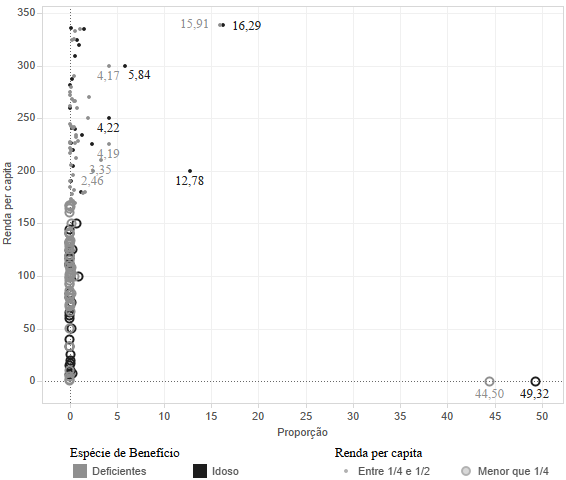
\includegraphics[]{distrbuicao_percapita.png}
	\begin{figure}[!h]
		\caption{Proporção de famílias por renda per capita }
		\label{rend_resumo_figura}
	\end{figure}
\end{center}

\section{Pobreza em grupos de estrato de renda per capita do BPC}

Uma análise individual dos indicadores de cada componente das seis dimensões não demonstra uma pior situação geral para nenhum dos estrados de rendas de interesse: há uma alternância de maior vulnerabilidade por grupos para cada indicador.  As questões mais relevantes para ambos grupos, que indicam vulnerabilidade,  são a ausência de cônjuge, baixa proporção de indivíduos em idade ativa,  baixo acesso ao conhecimento, má situação no acesso ao trabalho, não possuir computador, falta de planos de saúde e existência de membros com doenças crônicas. A baixa vulnerabilidade nos indicadores de desenvolvimento infantil, se deve a baixa ocorrência de crianças no domicílio.  A figura \ref{ind_resumo_figura} apresenta as proporções de famílias com vulnerabilidades nos indicadores apresentados, esses estão ordenador por dimensões. 

\begin{landscape}
\begin{center}
	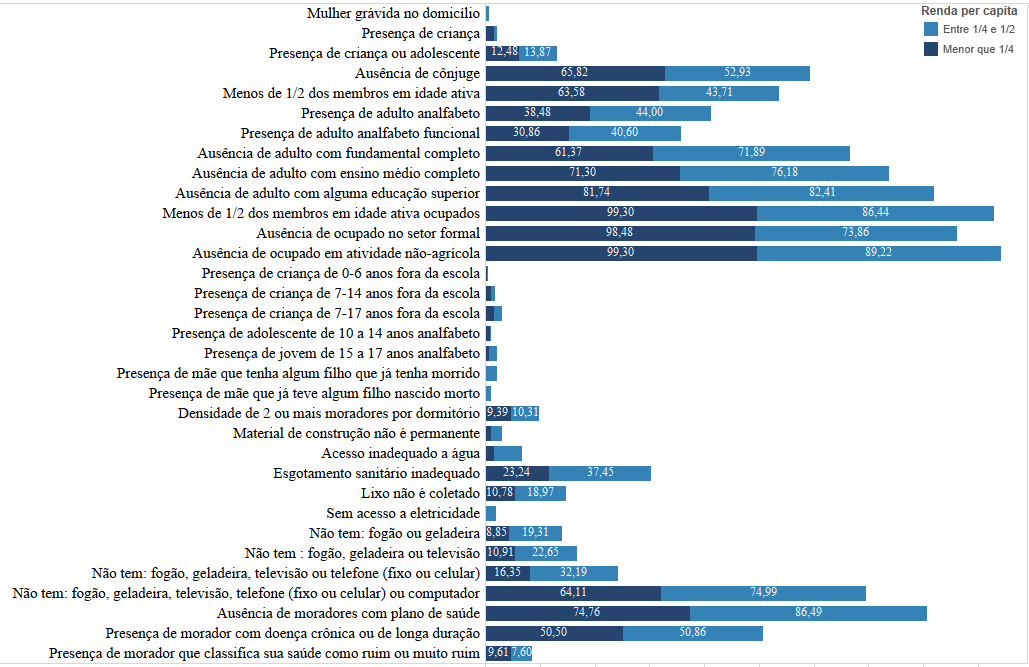
\includegraphics[width= 23cm, height=14.5cm ]{resumo_indicadores.png}
	\begin{figure}[!h]
		\caption{Proporção de famílias com vulnerabilidades nos indicadores de pobreza}
		\label{ind_resumo_figura}
	\end{figure}
\end{center}
\end{landscape}

Como mostra a tabela \ref{tab_graupobreza}, o grau de pobreza entre os estratos de renda \textit{per capita} são idênticos, ambos têm 40\% de pobreza. No entanto, há dimensões em que o um grupo pode ser considerado mais pobre e outro em que inverte-se a pobreza entre os grupos, embora essa diferença não ultrapasse os 7 ponto, exceto no caso de acesso ao trabalho, em que o estrato de renda \textit{per capita} abaixo de 1/4 tem uma condição de 15 ponto pior do que o outro estrato. 
 
 Mesmo considerando separadamente benefícios ao idoso e ao deficiente e por estrato de renda, a diferença entre o indicador geral não é tão relevante, variando em no máximo dois pontos. A maior diferença encontrada está entre os deficientes, sendo que os com renda maior que um quarto do salário mínimo estão em situação um pouco melhor do que os com renda menor que um quarto. Comparando todas as dimensões aferidas da pobreza, os dois grupos continuam similares, havendo alternância do estrato em pior situação nas dimensões. 

\begin{table}[H]
	\footnotesize
	\centering
	\caption{Grau multidimensional de pobreza -- estrato de renda per capita}
	\label{tab_graupobreza}
	\begin{tabular}{@{}m{5cm}lllllll@{}}
		\toprule
		\multirow{2}{*}{Dimensão} & \multirow{2}{*}{Total} & \multicolumn{2}{c}{Total}                                            & \multicolumn{2}{c}{Idoso}                                            & \multicolumn{2}{c}{Deficiente}                                       \\ \cmidrule(l){3-8} 
		&                        & Até 1/4 & \begin{tabular}[c]{@{}l@{}}Entre 1/4\\  e 1/2\end{tabular} & Até 1/4 & \begin{tabular}[c]{@{}l@{}}Entre 1/4\\  e 1/2\end{tabular} & Até 1/4 & \begin{tabular}[c]{@{}l@{}}Entre 1/4 \\ e 1/2\end{tabular} \\ \midrule
		Indicador Geral           & 40,3                   & 40,3    & 40,2                                                       & 40,7    & 42,5                                          & 39,8    & 37,8                                                       \\
		Vulnerabilidade           & 23,9                   & 24,2    & 19,1                                                       & 24,8    & 22,7                                          & 23,5    & 15,3                                                       \\
		Acesso ao conhecimento    & 53,5                   & 53,1    & 59,6                                                       & 60,9    & 68,5                                          & 44,3    & 50,4                                                       \\
		Acesso ao trabalho        & 98,1                   & 99,1    & 84,0                                                       & 98,9    & 88,3                                          & 99,4    & 79,6                                                       \\
		Desenvolvimento infantil  & 1,4                    & 1,3     & 2,0                                                        & 0,0     & 0,1                                           & 2,7     & 4,0                                                        \\
		Condições habitacionais   & 12,0                   & 11,5    & 18,6                                                       & 10,0    & 17,2                                          & 13,3    & 20,0                                                       \\
		Saúde                     & 52,8                   & 52,4    & 57,9                                                       & 49,4    & 58,2                                          & 55,8    & 57,5                                                       \\ \bottomrule
	\end{tabular}
\end{table}

Como os indicadores por grupos são médios, poderia haver uma diferença quanto ao total da população acumulada em níveis de pobreza. No entanto, mesmo essa comparação demostra uma similaridade entre estratos e espécie do benefício: 50\% das famílias mais pobres têm índices de pobreza em torno de 40\%, como mostra a figura \ref{ind_ac_figura}.

\begin{center}
	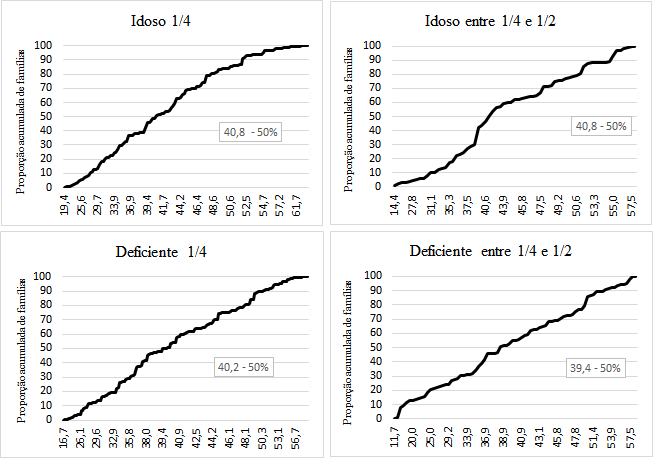
\includegraphics[scale=0.93]{prop_ac_indicegeral_especie.png}
	\begin{figure}[!h]
		\caption{Distribuiçã acumulada das famílias de acordo com o indicador de pobreza familiar}
		\label{ind_ac_figura}
	\end{figure}
\end{center}

% ---
% Conclusão
% ---
\chapter{Conclusão}

Em 2013 o Supremo Tribunal Federal (STF) julgou que, para o deferimento do
Benefício de prestação continuada, podem ser consideradas outros indicadores de miserabilidade além das regras existentes. Os demais critérios que comprovem a situação de miserabilidade do grupo familiar e da situação de vulnerabilidade carecem de regulamento e estão omitidos na Lei Orgânica de Assistência Social. Na pratica, o judiciário tem deferido o pedido do benefício para rendas \textit{per capita} de até meio salário mínimo. Dessa forma, o critério de pobreza para a concessão do benefício se tornou subjetivo, ficando à mercê da análise individual do judiciário.

O objetivo desse trabalho foi verificar se a pobreza entre os elegíveis ao BPC pela regra da LOAS e a adotada pelo judiciário são similares ou divergentes. Para isso, foi calculado um índice de pobreza multidimensional que levou em considerações dimensões comumente utilizadas nos estudos sobre o tema e comparado os dois estratos. 

Os resultados demostram que a pobreza medida pelo índice multidimensional dos dois grupos analisados não são diferentes. Além do mais, em algumas dimensões da pobreza, o estrato de renda superior a 1/4 está em pior situação do que o grupo naturalmente eleito no BPC. Se forem consideradas apenas o grau de miserabilidade, o resultados corroboram o entendimento do Supremo Tribunal Federal de que talvez os indivíduos com renda entre 1/4 e 1/2 devam ser incluídos no programa por entenderem que a pobreza entre eles não é tão diferente, mesmo com o dobro de renda por membro familiar. Outro ponto a ser destacado nos resultados é a também similaridade de pobreza entre grupos familiares de idosos e pessoas com deficiência. Atualmente, as regras do BPC tratam o cálculo da renda \textit{per capita} dos dois grupos de forma desigual, beneficiando os idosos ao nao inserir no calculo da renda familiar o rendimento de outro beneficiário idoso no mesmo domicílio. 

Como visto, a definição das variáveis e os pesos usados para compor um índice multidimensional de pobreza são basicamente empirismo advindo da disponibilidade da base de dados, sendo não trivial estimar o que as preferências sociais para definir as dimensões e seus pesos. Outro problema que se pode ter é que uma família pode ser pobre do ponto de vista de uma dimensão e não ser de outro. Embora tenha-se ciência de que a renda não é um perfeito indicador de pobreza, a operacionalização do programa a partir de corte de renda é mais facil. Dada a aferição da similaridade de pobreza nas diversas dimensões entre os dois cortes de renda, e a prática no judiciário de se considerar o corte de renda como de fato 1/2 do salário mínimo, a modificação da regra para esse mais alto limite traria maior previsibilidade ao programa sem reduzir a focalização na população mais pobre. 

% ----------------------------------------------------------
% ELEMENTOS PÓS-TEXTUAIS
% ----------------------------------------------------------
\postextual
% ----------------------------------------------------------

% ----------------------------------------------------------
% Referências bibliográficas
% ----------------------------------------------------------
\bibliography{bibliografia}

% ---
% Inicia os anexos
% ---
\begin{anexosenv}
	
	% Imprime uma página indicando o início dos anexos
	\partanexos
	
	% ---
	\chapter{Tabela verdade de recriação do grupamento familiar do BPC}
	\label{anexo_reclass}
	\footnotesize
	\begin{longtable}{@{}lcclc@{}}
			\toprule
			Condição do preeleito no domicilio        & Preeleito & Solteiro & Condição no domicílio (todos)                & Reclassificação \\ \midrule
			\endfirsthead
			\multicolumn{5}{c}%
			{\tablename\ \thetable\ -- \textit{Continuação da tabela}} \\
			\toprule
		Condição do preeleito no domicilio        & Preeleito & Solteiro & Condição no domicílio (todos)                 & Reclassificação \\ \midrule
			\endhead
			\hline \multicolumn{5}{r}{\textit{Continua na próxima página}} \\
			\endfoot
			\hline
			\endlastfoot
Pessoa responsável           & 1         & 1        & Pessoa responsável           & O Proprio       \\
Pessoa responsável           & 0         & 1        & Conjuge                      & Erro            \\
Pessoa responsável           & 0         & 1        & Filho(a) responsável/cônjuge & Filho           \\
Pessoa responsável           & 0         & 1        & Filho(a) responsável         & Filho           \\
Pessoa responsável           & 0         & 1        & Enteado(a)                   & Enteado         \\
Pessoa responsável           & 0         & 1        & Genro ou nora                & Erro            \\
Pessoa responsável           & 0         & 1        & Pai, mãe, padrasto/madrasta  & Pai/Mãe         \\
Pessoa responsável           & 0         & 1        & Sogro(a)                     & Não Entra       \\
Pessoa responsável           & 0         & 1        & Neto(a)                      & Não Entra       \\
Pessoa responsável           & 0         & 1        & Bisneto(a)                   & Não Entra       \\
Pessoa responsável           & 0         & 1        & Irmão ou irmã                & Irmao/Irma      \\
Pessoa responsável           & 0         & 1        & Avô ou avó                   & Não Entra       \\
Pessoa responsável           & 0         & 1        & Outros                       & Não Entra       \\
Conjuge                      & 0         & 1        & Pessoa responsável           & Erro            \\
Conjuge                      & 1         & 1        & Conjuge                      & Erro            \\
Conjuge                      & 0         & 1        & Filho(a) responsável/cônjuge & Filho           \\
Conjuge                      & 0         & 1        & Filho(a) responsável         & Enteado         \\
Conjuge                      & 0         & 1        & Enteado(a)                   & Filho           \\
Conjuge                      & 0         & 1        & Genro ou nora                & Erro            \\
Conjuge                      & 0         & 1        & Pai, mãe, padrasto/madrasta  & Não Entra       \\
Conjuge                      & 0         & 1        & Sogro(a)                     & Pai/Mãe         \\
Conjuge                      & 0         & 1        & Neto(a)                      & Não Entra       \\
Conjuge                      & 0         & 1        & Bisneto(a)                   & Não Entra       \\
Conjuge                      & 0         & 1        & Irmão ou irmã                & Não Entra       \\
Conjuge                      & 0         & 1        & Avô ou avó                   & Não Entra       \\
Conjuge                      & 0         & 1        & Outros                       & Ambiguo         \\
Filho(a) responsável/cônjuge & 1         & 1        & Filho(a) responsável/cônjuge & O Proprio       \\
Filho(a) responsável/cônjuge & 0         & 1        & Pessoa responsável           & Pai/Mãe         \\
Filho(a) responsável/cônjuge & 0         & 1        & Conjuge                      & Pai/Mãe         \\
Filho(a) responsável/cônjuge & 0         & 1        & Filho(a) responsável/cônjuge & Irmao/Irma      \\
Filho(a) responsável/cônjuge & 0         & 1        & Filho(a) responsável         & Irmao/Irma      \\
Filho(a) responsável/cônjuge & 0         & 1        & Enteado(a)                   & Irmao/Irma      \\
Filho(a) responsável/cônjuge & 0         & 1        & Genro ou nora                & Erro            \\
Filho(a) responsável/cônjuge & 0         & 1        & Pai, mãe, padrasto/madrasta  & Não Entra       \\
Filho(a) responsável/cônjuge & 0         & 1        & Sogro(a)                     & Não Entra       \\
Filho(a) responsável/cônjuge & 0         & 1        & Neto(a)                      & Ambiguo         \\
Filho(a) responsável/cônjuge & 0         & 1        & Bisneto(a)                   & Não Entra       \\
Filho(a) responsável/cônjuge & 0         & 1        & Irmão ou irmã                & Não Entra       \\
Filho(a) responsável/cônjuge & 0         & 1        & Avô ou avó                   & Não Entra       \\
Filho(a) responsável/cônjuge & 0         & 1        & Outros                       & Ambiguo         \\
Filho(a) responsável         & 1         & 1        & Filho(a) responsável         & O Proprio       \\
Filho(a) responsável         & 0         & 1        & Pessoa responsável           & Pai/Mãe         \\
Filho(a) responsável         & 0         & 1        & Conjuge                      & Pai/Mãe         \\
Filho(a) responsável         & 0         & 1        & Filho(a) responsável/cônjuge & Irmao/Irma      \\
Filho(a) responsável         & 0         & 1        & Filho(a) responsável         & Irmao/Irma      \\
Filho(a) responsável         & 0         & 1        & Enteado(a)                   & Irmao/Irma      \\
Filho(a) responsável         & 0         & 1        & Genro ou nora                & Erro            \\
Filho(a) responsável         & 0         & 1        & Pai, mãe, padrasto/madrasta  & Não Entra       \\
Filho(a) responsável         & 0         & 1        & Sogro(a)                     & Não Entra       \\
Filho(a) responsável         & 0         & 1        & Neto(a)                      & Ambiguo         \\
Filho(a) responsável         & 0         & 1        & Bisneto(a)                   & Não Entra       \\
Filho(a) responsável         & 0         & 1        & Irmão ou irmã                & Não Entra       \\
Filho(a) responsável         & 0         & 1        & Avô ou avó                   & Não Entra       \\
Filho(a) responsável         & 0         & 1        & Outros                       & Ambiguo         \\
Enteado(a)                   & 1         & 1        & Enteado(a)                   & O Proprio       \\
Enteado(a)                   & 0         & 1        & Pessoa responsável           & Pai/Mãe         \\
Enteado(a)                   & 0         & 1        & Conjuge                      & Erro            \\
Enteado(a)                   & 0         & 1        & Filho(a) responsável/cônjuge & Irmao/Irma      \\
Enteado(a)                   & 0         & 1        & Filho(a) responsável         & Irmao/Irma      \\
Enteado(a)                   & 0         & 1        & Enteado(a)                   & Irmao/Irma      \\
Enteado(a)                   & 0         & 1        & Genro ou nora                & Erro            \\
Enteado(a)                   & 0         & 1        & Pai, mãe, padrasto/madrasta  & Não Entra       \\
Enteado(a)                   & 0         & 1        & Sogro(a)                     & Não Entra       \\
Enteado(a)                   & 0         & 1        & Neto(a)                      & Ambiguo         \\
Enteado(a)                   & 0         & 1        & Bisneto(a)                   & Não Entra       \\
Enteado(a)                   & 0         & 1        & Irmão ou irmã                & Não Entra       \\
Enteado(a)                   & 0         & 1        & Avô ou avó                   & Não Entra       \\
Enteado(a)                   & 0         & 1        & Outros                       & Ambiguo         \\
Genro ou nora                & 1         & 1        & Genro ou nora                & Erro            \\
Genro ou nora                & 0         & 1        & Pessoa responsável           & Não Entra       \\
Genro ou nora                & 0         & 1        & Conjuge                      & Erro            \\
Genro ou nora                & 0         & 1        & Filho(a) responsável/cônjuge & Não Entra       \\
Genro ou nora                & 0         & 1        & Filho(a) responsável         & Não Entra       \\
Genro ou nora                & 0         & 1        & Enteado(a)                   & Não Entra       \\
Genro ou nora                & 0         & 1        & Genro ou nora                & Erro            \\
Genro ou nora                & 0         & 1        & Pai, mãe, padrasto/madrasta  & Não Entra       \\
Genro ou nora                & 0         & 1        & Sogro(a)                     & Não Entra       \\
Genro ou nora                & 0         & 1        & Neto(a)                      & Ambiguo         \\
Genro ou nora                & 0         & 1        & Bisneto(a)                   & Não Entra       \\
Genro ou nora                & 0         & 1        & Irmão ou irmã                & Não Entra       \\
Genro ou nora                & 0         & 1        & Avô ou avó                   & Não Entra       \\
Genro ou nora                & 0         & 1        & Outros                       & Ambiguo         \\
Pai, mãe, padrasto/madrasta  & 1         & 1        & Pai, mãe, padrasto/madrasta  & O Proprio       \\
Pai, mãe, padrasto/madrasta  & 0         & 1        & Pessoa responsável           & Filho           \\
Pai, mãe, padrasto/madrasta  & 0         & 1        & Conjuge                      & Erro            \\
Pai, mãe, padrasto/madrasta  & 0         & 1        & Filho(a) responsável/cônjuge & Não Entra       \\
Pai, mãe, padrasto/madrasta  & 0         & 1        & Filho(a) responsável         & Não Entra       \\
Pai, mãe, padrasto/madrasta  & 0         & 1        & Enteado(a)                   & Não Entra       \\
Pai, mãe, padrasto/madrasta  & 0         & 1        & Genro ou nora                & Não Entra       \\
Pai, mãe, padrasto/madrasta  & 0         & 1        & Pai, mãe, padrasto/madrasta  & Não Entra       \\
Pai, mãe, padrasto/madrasta  & 0         & 1        & Sogro(a)                     & Não Entra       \\
Pai, mãe, padrasto/madrasta  & 0         & 1        & Neto(a)                      & Não Entra       \\
Pai, mãe, padrasto/madrasta  & 0         & 1        & Bisneto(a)                   & Não Entra       \\
Pai, mãe, padrasto/madrasta  & 0         & 1        & Irmão ou irmã                & Filho           \\
Pai, mãe, padrasto/madrasta  & 0         & 1        & Avô ou avó                   & Pai/Mãe         \\
Pai, mãe, padrasto/madrasta  & 0         & 1        & Outros                       & Ambiguo         \\
Sogro(a)                     & 1         & 1        & Sogro(a)                     & O Proprio       \\
Sogro(a)                     & 0         & 1        & Pessoa responsável           & Não Entra       \\
Sogro(a)                     & 0         & 1        & Conjuge                      & Erro            \\
Sogro(a)                     & 0         & 1        & Filho(a) responsável/cônjuge & Não Entra       \\
Sogro(a)                     & 0         & 1        & Filho(a) responsável         & Não Entra       \\
Sogro(a)                     & 0         & 1        & Enteado(a)                   & Não Entra       \\
Sogro(a)                     & 0         & 1        & Genro ou nora                & Não Entra       \\
Sogro(a)                     & 0         & 1        & Pai, mãe, padrasto/madrasta  & Não Entra       \\
Sogro(a)                     & 0         & 1        & Sogro(a)                     & Não Entra       \\
Sogro(a)                     & 0         & 1        & Neto(a)                      & Não Entra       \\
Sogro(a)                     & 0         & 1        & Bisneto(a)                   & Não Entra       \\
Sogro(a)                     & 0         & 1        & Irmão ou irmã                & Não Entra       \\
Sogro(a)                     & 0         & 1        & Avô ou avó                   & Não Entra       \\
Sogro(a)                     & 0         & 1        & Outros                       & Ambiguo         \\
Neto(a)                      & 1         & 1        & Neto(a)                      & O Proprio       \\
Neto(a)                      & 0         & 1        & Pessoa responsável           & Não Entra       \\
Neto(a)                      & 0         & 1        & Conjuge                      & Erro            \\
Neto(a)                      & 0         & 1        & Filho(a) responsável/cônjuge & Ambiguo         \\
Neto(a)                      & 0         & 1        & Filho(a) responsável         & Ambiguo         \\
Neto(a)                      & 0         & 1        & Enteado(a)                   & Ambiguo         \\
Neto(a)                      & 0         & 1        & Genro ou nora                & Erro            \\
Neto(a)                      & 0         & 1        & Pai, mãe, padrasto/madrasta  & Não Entra       \\
Neto(a)                      & 0         & 1        & Sogro(a)                     & Não Entra       \\
Neto(a)                      & 0         & 1        & Neto(a)                      & Ambiguo         \\
Neto(a)                      & 0         & 1        & Bisneto(a)                   & Não Entra       \\
Neto(a)                      & 0         & 1        & Irmão ou irmã                & Não Entra       \\
Neto(a)                      & 0         & 1        & Avô ou avó                   & Não Entra       \\
Neto(a)                      & 0         & 1        & Outros                       & Ambiguo         \\
Bisneto(a)                   & 1         & 1        & Bisneto(a)                   & O Proprio       \\
Bisneto(a)                   & 0         & 1        & Pessoa responsável           & Não Entra       \\
Bisneto(a)                   & 0         & 1        & Conjuge                      & Erro            \\
Bisneto(a)                   & 0         & 1        & Filho(a) responsável/cônjuge & Não Entra       \\
Bisneto(a)                   & 0         & 1        & Filho(a) responsável         & Não Entra       \\
Bisneto(a)                   & 0         & 1        & Enteado(a)                   & Não Entra       \\
Bisneto(a)                   & 0         & 1        & Genro ou nora                & Erro            \\
Bisneto(a)                   & 0         & 1        & Pai, mãe, padrasto/madrasta  & Não Entra       \\
Bisneto(a)                   & 0         & 1        & Sogro(a)                     & Não Entra       \\
Bisneto(a)                   & 0         & 1        & Neto(a)                      & Ambiguo         \\
Bisneto(a)                   & 0         & 1        & Bisneto(a)                   & Ambiguo         \\
Bisneto(a)                   & 0         & 1        & Irmão ou irmã                & Não Entra       \\
Bisneto(a)                   & 0         & 1        & Avô ou avó                   & Não Entra       \\
Bisneto(a)                   & 0         & 1        & Outros                       & Ambiguo         \\
Irmão ou irmã                & 1         & 1        & Irmão ou irmã                & O Proprio       \\
Irmão ou irmã                & 0         & 1        & Pessoa responsável           & Irmao/Irma      \\
Irmão ou irmã                & 0         & 1        & Conjuge                      & Erro            \\
Irmão ou irmã                & 0         & 1        & Filho(a) responsável/cônjuge & Não Entra       \\
Irmão ou irmã                & 0         & 1        & Filho(a) responsável         & Não Entra       \\
Irmão ou irmã                & 0         & 1        & Enteado(a)                   & Não Entra       \\
Irmão ou irmã                & 0         & 1        & Genro ou nora                & Erro            \\
Irmão ou irmã                & 0         & 1        & Pai, mãe, padrasto/madrasta  & Pai/Mãe         \\
Irmão ou irmã                & 0         & 1        & Sogro(a)                     & Não Entra       \\
Irmão ou irmã                & 0         & 1        & Neto(a)                      & Não Entra       \\
Irmão ou irmã                & 0         & 1        & Bisneto(a)                   & Não Entra       \\
Irmão ou irmã                & 0         & 1        & Irmão ou irmã                & Irmao/Irma      \\
Irmão ou irmã                & 0         & 1        & Avô ou avó                   & Não Entra       \\
Irmão ou irmã                & 0         & 1        & Outros                       & Ambiguo         \\
Avô ou avó                   & 1         & 1        & Avô ou avó                   & O Proprio       \\
Avô ou avó                   & 0         & 1        & Pessoa responsável           & Não Entra       \\
Avô ou avó                   & 0         & 1        & Conjuge                      & Erro            \\
Avô ou avó                   & 0         & 1        & Filho(a) responsável/cônjuge & Não Entra       \\
Avô ou avó                   & 0         & 1        & Filho(a) responsável         & Não Entra       \\
Avô ou avó                   & 0         & 1        & Enteado(a)                   & Não Entra       \\
Avô ou avó                   & 0         & 1        & Genro ou nora                & Erro            \\
Avô ou avó                   & 0         & 1        & Pai, mãe, padrasto/madrasta  & Ambiguo         \\
Avô ou avó                   & 0         & 1        & Sogro(a)                     & Não Entra       \\
Avô ou avó                   & 0         & 1        & Neto(a)                      & Não Entra       \\
Avô ou avó                   & 0         & 1        & Bisneto(a)                   & Não Entra       \\
Avô ou avó                   & 0         & 1        & Irmão ou irmã                & Não Entra       \\
Avô ou avó                   & 0         & 1        & Avô ou avó                   & Não Entra       \\
Avô ou avó                   & 0         & 1        & Outros                       & Ambiguo         \\
Outros                       & 1         & 1        & Outros                       & O Proprio       \\
Outros                       & 0         & 1        & Pessoa responsável           & Não Entra       \\
Outros                       & 0         & 1        & Conjuge                      & Erro            \\
Outros                       & 0         & 1        & Filho(a) responsável/cônjuge & Ambiguo         \\
Outros                       & 0         & 1        & Filho(a) responsável         & Ambiguo         \\
Outros                       & 0         & 1        & Enteado(a)                   & Ambiguo         \\
Outros                       & 0         & 1        & Genro ou nora                & Erro            \\
Outros                       & 0         & 1        & Pai, mãe, padrasto/madrasta  & Ambiguo         \\
Outros                       & 0         & 1        & Sogro(a)                     & Ambiguo         \\
Outros                       & 0         & 1        & Neto(a)                      & Ambiguo         \\
Outros                       & 0         & 1        & Bisneto(a)                   & Ambiguo         \\
Outros                       & 0         & 1        & Irmão ou irmã                & Ambiguo         \\
Outros                       & 0         & 1        & Avô ou avó                   & Ambiguo         \\
Outros                       & 0         & 1        & Outros                       & Ambiguo         \\
Pessoa responsável           & 1         & 0        & Pessoa responsável           & O Proprio       \\
Pessoa responsável           & 0         & 0        & Conjuge                      & Conjuge         \\
Pessoa responsável           & 0         & 0        & Filho(a) responsável/cônjuge & Não Entra       \\
Pessoa responsável           & 0         & 0        & Filho(a) responsável         & Não Entra       \\
Pessoa responsável           & 0         & 0        & Enteado(a)                   & Não Entra       \\
Pessoa responsável           & 0         & 0        & Genro ou nora                & Não Entra       \\
Pessoa responsável           & 0         & 0        & Pai, mãe, padrasto/madrasta  & Pai/Mãe         \\
Pessoa responsável           & 0         & 0        & Sogro(a)                     & Não Entra       \\
Pessoa responsável           & 0         & 0        & Neto(a)                      & Não Entra       \\
Pessoa responsável           & 0         & 0        & Bisneto(a)                   & Não Entra       \\
Pessoa responsável           & 0         & 0        & Irmão ou irmã                & Não Entra       \\
Pessoa responsável           & 0         & 0        & Avô ou avó                   & Não Entra       \\
Pessoa responsável           & 0         & 0        & Outros                       & Não Entra       \\
Conjuge                      & 0         & 0        & Pessoa responsável           & Conjuge         \\
Conjuge                      & 1         & 0        & Conjuge                      & O Proprio       \\
Conjuge                      & 0         & 0        & Filho(a) responsável/cônjuge & Não Entra       \\
Conjuge                      & 0         & 0        & Filho(a) responsável         & Não Entra       \\
Conjuge                      & 0         & 0        & Enteado(a)                   & Não Entra       \\
Conjuge                      & 0         & 0        & Genro ou nora                & Não Entra       \\
Conjuge                      & 0         & 0        & Pai, mãe, padrasto/madrasta  & Não Entra       \\
Conjuge                      & 0         & 0        & Sogro(a)                     & Pai/Mãe         \\
Conjuge                      & 0         & 0        & Neto(a)                      & Não Entra       \\
Conjuge                      & 0         & 0        & Bisneto(a)                   & Não Entra       \\
Conjuge                      & 0         & 0        & Irmão ou irmã                & Não Entra       \\
Conjuge                      & 0         & 0        & Avô ou avó                   & Não Entra       \\
Conjuge                      & 0         & 0        & Outros                       & Ambiguo         \\
Filho(a) responsável/cônjuge & 1         & 0        & Filho(a) responsável/cônjuge & O Proprio       \\
Filho(a) responsável/cônjuge & 0         & 0        & Pessoa responsável           & Pai/Mãe         \\
Filho(a) responsável/cônjuge & 0         & 0        & Conjuge                      & Pai/Mãe         \\
Filho(a) responsável/cônjuge & 0         & 0        & Filho(a) responsável/cônjuge & Não Entra       \\
Filho(a) responsável/cônjuge & 0         & 0        & Filho(a) responsável         & Não Entra       \\
Filho(a) responsável/cônjuge & 0         & 0        & Enteado(a)                   & Não Entra       \\
Filho(a) responsável/cônjuge & 0         & 0        & Genro ou nora                & Ambiguo         \\
Filho(a) responsável/cônjuge & 0         & 0        & Pai, mãe, padrasto/madrasta  & Não Entra       \\
Filho(a) responsável/cônjuge & 0         & 0        & Sogro(a)                     & Não Entra       \\
Filho(a) responsável/cônjuge & 0         & 0        & Neto(a)                      & Não Entra       \\
Filho(a) responsável/cônjuge & 0         & 0        & Bisneto(a)                   & Não Entra       \\
Filho(a) responsável/cônjuge & 0         & 0        & Irmão ou irmã                & Não Entra       \\
Filho(a) responsável/cônjuge & 0         & 0        & Avô ou avó                   & Não Entra       \\
Filho(a) responsável/cônjuge & 0         & 0        & Outros                       & Ambiguo         \\
Filho(a) responsável         & 1         & 0        & Filho(a) responsável         & O Proprio       \\
Filho(a) responsável         & 0         & 0        & Pessoa responsável           & Pai/Mãe         \\
Filho(a) responsável         & 0         & 0        & Conjuge                      & Pai/Mãe         \\
Filho(a) responsável         & 0         & 0        & Filho(a) responsável/cônjuge & Não Entra       \\
Filho(a) responsável         & 0         & 0        & Filho(a) responsável         & Não Entra       \\
Filho(a) responsável         & 0         & 0        & Enteado(a)                   & Não Entra       \\
Filho(a) responsável         & 0         & 0        & Genro ou nora                & Ambiguo         \\
Filho(a) responsável         & 0         & 0        & Pai, mãe, padrasto/madrasta  & Não Entra       \\
Filho(a) responsável         & 0         & 0        & Sogro(a)                     & Não Entra       \\
Filho(a) responsável         & 0         & 0        & Neto(a)                      & Não Entra       \\
Filho(a) responsável         & 0         & 0        & Bisneto(a)                   & Não Entra       \\
Filho(a) responsável         & 0         & 0        & Irmão ou irmã                & Não Entra       \\
Filho(a) responsável         & 0         & 0        & Avô ou avó                   & Não Entra       \\
Filho(a) responsável         & 0         & 0        & Outros                       & Ambiguo         \\
Enteado(a)                   & 1         & 0        & Enteado(a)                   & O Proprio       \\
Enteado(a)                   & 0         & 0        & Pessoa responsável           & Pai/Mãe         \\
Enteado(a)                   & 0         & 0        & Conjuge                      & Ambiguo         \\
Enteado(a)                   & 0         & 0        & Filho(a) responsável/cônjuge & Não Entra       \\
Enteado(a)                   & 0         & 0        & Filho(a) responsável         & Não Entra       \\
Enteado(a)                   & 0         & 0        & Enteado(a)                   & Não Entra       \\
Enteado(a)                   & 0         & 0        & Genro ou nora                & Não Entra       \\
Enteado(a)                   & 0         & 0        & Pai, mãe, padrasto/madrasta  & Não Entra       \\
Enteado(a)                   & 0         & 0        & Sogro(a)                     & Não Entra       \\
Enteado(a)                   & 0         & 0        & Neto(a)                      & Não Entra       \\
Enteado(a)                   & 0         & 0        & Bisneto(a)                   & Não Entra       \\
Enteado(a)                   & 0         & 0        & Irmão ou irmã                & Não Entra       \\
Enteado(a)                   & 0         & 0        & Avô ou avó                   & Não Entra       \\
Enteado(a)                   & 0         & 0        & Outros                       & Ambiguo         \\
Genro ou nora                & 1         & 0        & Genro ou nora                & O Proprio       \\
Genro ou nora                & 0         & 0        & Pessoa responsável           & Não Entra       \\
Genro ou nora                & 0         & 0        & Conjuge                      & Não Entra       \\
Genro ou nora                & 0         & 0        & Filho(a) responsável/cônjuge & Ambiguo         \\
Genro ou nora                & 0         & 0        & Filho(a) responsável         & Ambiguo         \\
Genro ou nora                & 0         & 0        & Enteado(a)                   & Ambiguo         \\
Genro ou nora                & 0         & 0        & Genro ou nora                & Não Entra       \\
Genro ou nora                & 0         & 0        & Pai, mãe, padrasto/madrasta  & Não Entra       \\
Genro ou nora                & 0         & 0        & Sogro(a)                     & Não Entra       \\
Genro ou nora                & 0         & 0        & Neto(a)                      & Não Entra       \\
Genro ou nora                & 0         & 0        & Bisneto(a)                   & Não Entra       \\
Genro ou nora                & 0         & 0        & Irmão ou irmã                & Não Entra       \\
Genro ou nora                & 0         & 0        & Avô ou avó                   & Não Entra       \\
Genro ou nora                & 0         & 0        & Outros                       & Ambiguo         \\
Pai, mãe, padrasto/madrasta  & 1         & 0        & Pai, mãe, padrasto/madrasta  & O Proprio       \\
Pai, mãe, padrasto/madrasta  & 0         & 0        & Pessoa responsável           & Não Entra       \\
Pai, mãe, padrasto/madrasta  & 0         & 0        & Conjuge                      & Não Entra       \\
Pai, mãe, padrasto/madrasta  & 0         & 0        & Filho(a) responsável/cônjuge & Não Entra       \\
Pai, mãe, padrasto/madrasta  & 0         & 0        & Filho(a) responsável         & Não Entra       \\
Pai, mãe, padrasto/madrasta  & 0         & 0        & Enteado(a)                   & Não Entra       \\
Pai, mãe, padrasto/madrasta  & 0         & 0        & Genro ou nora                & Não Entra       \\
Pai, mãe, padrasto/madrasta  & 0         & 0        & Pai, mãe, padrasto/madrasta  & Conjuge         \\
Pai, mãe, padrasto/madrasta  & 0         & 0        & Sogro(a)                     & Não Entra       \\
Pai, mãe, padrasto/madrasta  & 0         & 0        & Neto(a)                      & Não Entra       \\
Pai, mãe, padrasto/madrasta  & 0         & 0        & Bisneto(a)                   & Não Entra       \\
Pai, mãe, padrasto/madrasta  & 0         & 0        & Irmão ou irmã                & Não Entra       \\
Pai, mãe, padrasto/madrasta  & 0         & 0        & Avô ou avó                   & Pai/Mãe         \\
Pai, mãe, padrasto/madrasta  & 0         & 0        & Outros                       & Ambiguo         \\
Sogro(a)                     & 1         & 0        & Sogro(a)                     & O Proprio       \\
Sogro(a)                     & 0         & 0        & Pessoa responsável           & Não Entra       \\
Sogro(a)                     & 0         & 0        & Conjuge                      & Não Entra       \\
Sogro(a)                     & 0         & 0        & Filho(a) responsável/cônjuge & Não Entra       \\
Sogro(a)                     & 0         & 0        & Filho(a) responsável         & Não Entra       \\
Sogro(a)                     & 0         & 0        & Enteado(a)                   & Não Entra       \\
Sogro(a)                     & 0         & 0        & Genro ou nora                & Não Entra       \\
Sogro(a)                     & 0         & 0        & Pai, mãe, padrasto/madrasta  & Não Entra       \\
Sogro(a)                     & 0         & 0        & Sogro(a)                     & Conjuge         \\
Sogro(a)                     & 0         & 0        & Neto(a)                      & Não Entra       \\
Sogro(a)                     & 0         & 0        & Bisneto(a)                   & Não Entra       \\
Sogro(a)                     & 0         & 0        & Irmão ou irmã                & Não Entra       \\
Sogro(a)                     & 0         & 0        & Avô ou avó                   & Não Entra       \\
Sogro(a)                     & 0         & 0        & Outros                       & Ambiguo         \\
Neto(a)                      & 1         & 0        & Neto(a)                      & O Proprio       \\
Neto(a)                      & 0         & 0        & Pessoa responsável           & Não Entra       \\
Neto(a)                      & 0         & 0        & Conjuge                      & Não Entra       \\
Neto(a)                      & 0         & 0        & Filho(a) responsável/cônjuge & Ambiguo         \\
Neto(a)                      & 0         & 0        & Filho(a) responsável         & Ambiguo         \\
Neto(a)                      & 0         & 0        & Enteado(a)                   & Ambiguo         \\
Neto(a)                      & 0         & 0        & Genro ou nora                & Ambiguo         \\
Neto(a)                      & 0         & 0        & Pai, mãe, padrasto/madrasta  & Não Entra       \\
Neto(a)                      & 0         & 0        & Sogro(a)                     & Não Entra       \\
Neto(a)                      & 0         & 0        & Neto(a)                      & Não Entra       \\
Neto(a)                      & 0         & 0        & Bisneto(a)                   & Não Entra       \\
Neto(a)                      & 0         & 0        & Irmão ou irmã                & Não Entra       \\
Neto(a)                      & 0         & 0        & Avô ou avó                   & Não Entra       \\
Neto(a)                      & 0         & 0        & Outros                       & Ambiguo         \\
Bisneto(a)                   & 1         & 0        & Bisneto(a)                   & O Proprio       \\
Bisneto(a)                   & 0         & 0        & Pessoa responsável           & Não Entra       \\
Bisneto(a)                   & 0         & 0        & Conjuge                      & Não Entra       \\
Bisneto(a)                   & 0         & 0        & Filho(a) responsável/cônjuge & Não Entra       \\
Bisneto(a)                   & 0         & 0        & Filho(a) responsável         & Não Entra       \\
Bisneto(a)                   & 0         & 0        & Enteado(a)                   & Não Entra       \\
Bisneto(a)                   & 0         & 0        & Genro ou nora                & Não Entra       \\
Bisneto(a)                   & 0         & 0        & Pai, mãe, padrasto/madrasta  & Não Entra       \\
Bisneto(a)                   & 0         & 0        & Sogro(a)                     & Não Entra       \\
Bisneto(a)                   & 0         & 0        & Neto(a)                      & Ambiguo         \\
Bisneto(a)                   & 0         & 0        & Bisneto(a)                   & Não Entra       \\
Bisneto(a)                   & 0         & 0        & Irmão ou irmã                & Não Entra       \\
Bisneto(a)                   & 0         & 0        & Avô ou avó                   & Não Entra       \\
Bisneto(a)                   & 0         & 0        & Outros                       & Ambiguo         \\
Irmão ou irmã                & 1         & 0        & Irmão ou irmã                & O Proprio       \\
Irmão ou irmã                & 0         & 0        & Pessoa responsável           & Não Entra       \\
Irmão ou irmã                & 0         & 0        & Conjuge                      & Não Entra       \\
Irmão ou irmã                & 0         & 0        & Filho(a) responsável/cônjuge & Não Entra       \\
Irmão ou irmã                & 0         & 0        & Filho(a) responsável         & Não Entra       \\
Irmão ou irmã                & 0         & 0        & Enteado(a)                   & Não Entra       \\
Irmão ou irmã                & 0         & 0        & Genro ou nora                & Não Entra       \\
Irmão ou irmã                & 0         & 0        & Pai, mãe, padrasto/madrasta  & Pai/Mãe         \\
Irmão ou irmã                & 0         & 0        & Sogro(a)                     & Não Entra       \\
Irmão ou irmã                & 0         & 0        & Neto(a)                      & Não Entra       \\
Irmão ou irmã                & 0         & 0        & Bisneto(a)                   & Não Entra       \\
Irmão ou irmã                & 0         & 0        & Irmão ou irmã                & Não Entra       \\
Irmão ou irmã                & 0         & 0        & Avô ou avó                   & Não Entra       \\
Irmão ou irmã                & 0         & 0        & Outros                       & Ambiguo         \\
Avô ou avó                   & 1         & 0        & Avô ou avó                   & O Proprio       \\
Avô ou avó                   & 0         & 0        & Pessoa responsável           & Não Entra       \\
Avô ou avó                   & 0         & 0        & Conjuge                      & Não Entra       \\
Avô ou avó                   & 0         & 0        & Filho(a) responsável/cônjuge & Não Entra       \\
Avô ou avó                   & 0         & 0        & Filho(a) responsável         & Não Entra       \\
Avô ou avó                   & 0         & 0        & Enteado(a)                   & Não Entra       \\
Avô ou avó                   & 0         & 0        & Genro ou nora                & Não Entra       \\
Avô ou avó                   & 0         & 0        & Pai, mãe, padrasto/madrasta  & Ambiguo         \\
Avô ou avó                   & 0         & 0        & Sogro(a)                     & Não Entra       \\
Avô ou avó                   & 0         & 0        & Neto(a)                      & Não Entra       \\
Avô ou avó                   & 0         & 0        & Bisneto(a)                   & Não Entra       \\
Avô ou avó                   & 0         & 0        & Irmão ou irmã                & Não Entra       \\
Avô ou avó                   & 0         & 0        & Avô ou avó                   & Ambiguo         \\
Avô ou avó                   & 0         & 0        & Outros                       & Ambiguo         \\
Outros                       & 1         & 0        & Outros                       & O Proprio       \\
Outros                       & 0         & 0        & Pessoa responsável           & Não Entra       \\
Outros                       & 0         & 0        & Conjuge                      & Ambiguo         \\
Outros                       & 0         & 0        & Filho(a) responsável/cônjuge & Ambiguo         \\
Outros                       & 0         & 0        & Filho(a) responsável         & Ambiguo         \\
Outros                       & 0         & 0        & Enteado(a)                   & Ambiguo         \\
Outros                       & 0         & 0        & Genro ou nora                & Ambiguo         \\
Outros                       & 0         & 0        & Pai, mãe, padrasto/madrasta  & Ambiguo         \\
Outros                       & 0         & 0        & Sogro(a)                     & Ambiguo         \\
Outros                       & 0         & 0        & Neto(a)                      & Ambiguo         \\
Outros                       & 0         & 0        & Bisneto(a)                   & Ambiguo         \\
Outros                       & 0         & 0        & Irmão ou irmã                & Ambiguo         \\
Outros                       & 0         & 0        & Avô ou avó                   & Ambiguo         \\
Outros                       & 0         & 0        & Outros                       & Ambiguo         \\ \bottomrule
\end{longtable}
	% ---
	
	
\end{anexosenv}


%---------------------------------------------------------------------
% INDICE REMISSIVO
%---------------------------------------------------------------------
\phantompart
\printindex
%---------------------------------------------------------------------

\end{document}
